% Generated by Sphinx.
\def\sphinxdocclass{report}
\documentclass[letterpaper,10pt,english]{sphinxmanual}
\usepackage[utf8]{inputenc}
\DeclareUnicodeCharacter{00A0}{\nobreakspace}
\usepackage{cmap}
\usepackage[T1]{fontenc}
\usepackage{babel}
\usepackage{times}
\usepackage[Bjarne]{fncychap}
\usepackage{longtable}
\usepackage{sphinx}
\usepackage{multirow}


\title{draft1 Documentation}
\date{January 30, 2015}
\release{0.1}
\author{Shotaro Fujimoto}
\newcommand{\sphinxlogo}{}
\renewcommand{\releasename}{Release}
\makeindex

\makeatletter
\def\PYG@reset{\let\PYG@it=\relax \let\PYG@bf=\relax%
    \let\PYG@ul=\relax \let\PYG@tc=\relax%
    \let\PYG@bc=\relax \let\PYG@ff=\relax}
\def\PYG@tok#1{\csname PYG@tok@#1\endcsname}
\def\PYG@toks#1+{\ifx\relax#1\empty\else%
    \PYG@tok{#1}\expandafter\PYG@toks\fi}
\def\PYG@do#1{\PYG@bc{\PYG@tc{\PYG@ul{%
    \PYG@it{\PYG@bf{\PYG@ff{#1}}}}}}}
\def\PYG#1#2{\PYG@reset\PYG@toks#1+\relax+\PYG@do{#2}}

\expandafter\def\csname PYG@tok@gd\endcsname{\def\PYG@tc##1{\textcolor[rgb]{0.63,0.00,0.00}{##1}}}
\expandafter\def\csname PYG@tok@gu\endcsname{\let\PYG@bf=\textbf\def\PYG@tc##1{\textcolor[rgb]{0.50,0.00,0.50}{##1}}}
\expandafter\def\csname PYG@tok@gt\endcsname{\def\PYG@tc##1{\textcolor[rgb]{0.00,0.27,0.87}{##1}}}
\expandafter\def\csname PYG@tok@gs\endcsname{\let\PYG@bf=\textbf}
\expandafter\def\csname PYG@tok@gr\endcsname{\def\PYG@tc##1{\textcolor[rgb]{1.00,0.00,0.00}{##1}}}
\expandafter\def\csname PYG@tok@cm\endcsname{\let\PYG@it=\textit\def\PYG@tc##1{\textcolor[rgb]{0.25,0.50,0.56}{##1}}}
\expandafter\def\csname PYG@tok@vg\endcsname{\def\PYG@tc##1{\textcolor[rgb]{0.73,0.38,0.84}{##1}}}
\expandafter\def\csname PYG@tok@m\endcsname{\def\PYG@tc##1{\textcolor[rgb]{0.13,0.50,0.31}{##1}}}
\expandafter\def\csname PYG@tok@mh\endcsname{\def\PYG@tc##1{\textcolor[rgb]{0.13,0.50,0.31}{##1}}}
\expandafter\def\csname PYG@tok@cs\endcsname{\def\PYG@tc##1{\textcolor[rgb]{0.25,0.50,0.56}{##1}}\def\PYG@bc##1{\setlength{\fboxsep}{0pt}\colorbox[rgb]{1.00,0.94,0.94}{\strut ##1}}}
\expandafter\def\csname PYG@tok@ge\endcsname{\let\PYG@it=\textit}
\expandafter\def\csname PYG@tok@vc\endcsname{\def\PYG@tc##1{\textcolor[rgb]{0.73,0.38,0.84}{##1}}}
\expandafter\def\csname PYG@tok@il\endcsname{\def\PYG@tc##1{\textcolor[rgb]{0.13,0.50,0.31}{##1}}}
\expandafter\def\csname PYG@tok@go\endcsname{\def\PYG@tc##1{\textcolor[rgb]{0.20,0.20,0.20}{##1}}}
\expandafter\def\csname PYG@tok@cp\endcsname{\def\PYG@tc##1{\textcolor[rgb]{0.00,0.44,0.13}{##1}}}
\expandafter\def\csname PYG@tok@gi\endcsname{\def\PYG@tc##1{\textcolor[rgb]{0.00,0.63,0.00}{##1}}}
\expandafter\def\csname PYG@tok@gh\endcsname{\let\PYG@bf=\textbf\def\PYG@tc##1{\textcolor[rgb]{0.00,0.00,0.50}{##1}}}
\expandafter\def\csname PYG@tok@ni\endcsname{\let\PYG@bf=\textbf\def\PYG@tc##1{\textcolor[rgb]{0.84,0.33,0.22}{##1}}}
\expandafter\def\csname PYG@tok@nl\endcsname{\let\PYG@bf=\textbf\def\PYG@tc##1{\textcolor[rgb]{0.00,0.13,0.44}{##1}}}
\expandafter\def\csname PYG@tok@nn\endcsname{\let\PYG@bf=\textbf\def\PYG@tc##1{\textcolor[rgb]{0.05,0.52,0.71}{##1}}}
\expandafter\def\csname PYG@tok@no\endcsname{\def\PYG@tc##1{\textcolor[rgb]{0.38,0.68,0.84}{##1}}}
\expandafter\def\csname PYG@tok@na\endcsname{\def\PYG@tc##1{\textcolor[rgb]{0.25,0.44,0.63}{##1}}}
\expandafter\def\csname PYG@tok@nb\endcsname{\def\PYG@tc##1{\textcolor[rgb]{0.00,0.44,0.13}{##1}}}
\expandafter\def\csname PYG@tok@nc\endcsname{\let\PYG@bf=\textbf\def\PYG@tc##1{\textcolor[rgb]{0.05,0.52,0.71}{##1}}}
\expandafter\def\csname PYG@tok@nd\endcsname{\let\PYG@bf=\textbf\def\PYG@tc##1{\textcolor[rgb]{0.33,0.33,0.33}{##1}}}
\expandafter\def\csname PYG@tok@ne\endcsname{\def\PYG@tc##1{\textcolor[rgb]{0.00,0.44,0.13}{##1}}}
\expandafter\def\csname PYG@tok@nf\endcsname{\def\PYG@tc##1{\textcolor[rgb]{0.02,0.16,0.49}{##1}}}
\expandafter\def\csname PYG@tok@si\endcsname{\let\PYG@it=\textit\def\PYG@tc##1{\textcolor[rgb]{0.44,0.63,0.82}{##1}}}
\expandafter\def\csname PYG@tok@s2\endcsname{\def\PYG@tc##1{\textcolor[rgb]{0.25,0.44,0.63}{##1}}}
\expandafter\def\csname PYG@tok@vi\endcsname{\def\PYG@tc##1{\textcolor[rgb]{0.73,0.38,0.84}{##1}}}
\expandafter\def\csname PYG@tok@nt\endcsname{\let\PYG@bf=\textbf\def\PYG@tc##1{\textcolor[rgb]{0.02,0.16,0.45}{##1}}}
\expandafter\def\csname PYG@tok@nv\endcsname{\def\PYG@tc##1{\textcolor[rgb]{0.73,0.38,0.84}{##1}}}
\expandafter\def\csname PYG@tok@s1\endcsname{\def\PYG@tc##1{\textcolor[rgb]{0.25,0.44,0.63}{##1}}}
\expandafter\def\csname PYG@tok@gp\endcsname{\let\PYG@bf=\textbf\def\PYG@tc##1{\textcolor[rgb]{0.78,0.36,0.04}{##1}}}
\expandafter\def\csname PYG@tok@sh\endcsname{\def\PYG@tc##1{\textcolor[rgb]{0.25,0.44,0.63}{##1}}}
\expandafter\def\csname PYG@tok@ow\endcsname{\let\PYG@bf=\textbf\def\PYG@tc##1{\textcolor[rgb]{0.00,0.44,0.13}{##1}}}
\expandafter\def\csname PYG@tok@sx\endcsname{\def\PYG@tc##1{\textcolor[rgb]{0.78,0.36,0.04}{##1}}}
\expandafter\def\csname PYG@tok@bp\endcsname{\def\PYG@tc##1{\textcolor[rgb]{0.00,0.44,0.13}{##1}}}
\expandafter\def\csname PYG@tok@c1\endcsname{\let\PYG@it=\textit\def\PYG@tc##1{\textcolor[rgb]{0.25,0.50,0.56}{##1}}}
\expandafter\def\csname PYG@tok@kc\endcsname{\let\PYG@bf=\textbf\def\PYG@tc##1{\textcolor[rgb]{0.00,0.44,0.13}{##1}}}
\expandafter\def\csname PYG@tok@c\endcsname{\let\PYG@it=\textit\def\PYG@tc##1{\textcolor[rgb]{0.25,0.50,0.56}{##1}}}
\expandafter\def\csname PYG@tok@mf\endcsname{\def\PYG@tc##1{\textcolor[rgb]{0.13,0.50,0.31}{##1}}}
\expandafter\def\csname PYG@tok@err\endcsname{\def\PYG@bc##1{\setlength{\fboxsep}{0pt}\fcolorbox[rgb]{1.00,0.00,0.00}{1,1,1}{\strut ##1}}}
\expandafter\def\csname PYG@tok@mb\endcsname{\def\PYG@tc##1{\textcolor[rgb]{0.13,0.50,0.31}{##1}}}
\expandafter\def\csname PYG@tok@ss\endcsname{\def\PYG@tc##1{\textcolor[rgb]{0.32,0.47,0.09}{##1}}}
\expandafter\def\csname PYG@tok@sr\endcsname{\def\PYG@tc##1{\textcolor[rgb]{0.14,0.33,0.53}{##1}}}
\expandafter\def\csname PYG@tok@mo\endcsname{\def\PYG@tc##1{\textcolor[rgb]{0.13,0.50,0.31}{##1}}}
\expandafter\def\csname PYG@tok@kd\endcsname{\let\PYG@bf=\textbf\def\PYG@tc##1{\textcolor[rgb]{0.00,0.44,0.13}{##1}}}
\expandafter\def\csname PYG@tok@mi\endcsname{\def\PYG@tc##1{\textcolor[rgb]{0.13,0.50,0.31}{##1}}}
\expandafter\def\csname PYG@tok@kn\endcsname{\let\PYG@bf=\textbf\def\PYG@tc##1{\textcolor[rgb]{0.00,0.44,0.13}{##1}}}
\expandafter\def\csname PYG@tok@o\endcsname{\def\PYG@tc##1{\textcolor[rgb]{0.40,0.40,0.40}{##1}}}
\expandafter\def\csname PYG@tok@kr\endcsname{\let\PYG@bf=\textbf\def\PYG@tc##1{\textcolor[rgb]{0.00,0.44,0.13}{##1}}}
\expandafter\def\csname PYG@tok@s\endcsname{\def\PYG@tc##1{\textcolor[rgb]{0.25,0.44,0.63}{##1}}}
\expandafter\def\csname PYG@tok@kp\endcsname{\def\PYG@tc##1{\textcolor[rgb]{0.00,0.44,0.13}{##1}}}
\expandafter\def\csname PYG@tok@w\endcsname{\def\PYG@tc##1{\textcolor[rgb]{0.73,0.73,0.73}{##1}}}
\expandafter\def\csname PYG@tok@kt\endcsname{\def\PYG@tc##1{\textcolor[rgb]{0.56,0.13,0.00}{##1}}}
\expandafter\def\csname PYG@tok@sc\endcsname{\def\PYG@tc##1{\textcolor[rgb]{0.25,0.44,0.63}{##1}}}
\expandafter\def\csname PYG@tok@sb\endcsname{\def\PYG@tc##1{\textcolor[rgb]{0.25,0.44,0.63}{##1}}}
\expandafter\def\csname PYG@tok@k\endcsname{\let\PYG@bf=\textbf\def\PYG@tc##1{\textcolor[rgb]{0.00,0.44,0.13}{##1}}}
\expandafter\def\csname PYG@tok@se\endcsname{\let\PYG@bf=\textbf\def\PYG@tc##1{\textcolor[rgb]{0.25,0.44,0.63}{##1}}}
\expandafter\def\csname PYG@tok@sd\endcsname{\let\PYG@it=\textit\def\PYG@tc##1{\textcolor[rgb]{0.25,0.44,0.63}{##1}}}

\def\PYGZbs{\char`\\}
\def\PYGZus{\char`\_}
\def\PYGZob{\char`\{}
\def\PYGZcb{\char`\}}
\def\PYGZca{\char`\^}
\def\PYGZam{\char`\&}
\def\PYGZlt{\char`\<}
\def\PYGZgt{\char`\>}
\def\PYGZsh{\char`\#}
\def\PYGZpc{\char`\%}
\def\PYGZdl{\char`\$}
\def\PYGZhy{\char`\-}
\def\PYGZsq{\char`\'}
\def\PYGZdq{\char`\"}
\def\PYGZti{\char`\~}
% for compatibility with earlier versions
\def\PYGZat{@}
\def\PYGZlb{[}
\def\PYGZrb{]}
\makeatother

\begin{document}

\maketitle
\tableofcontents
\phantomsection\label{index::doc}



\chapter{効率とシステムサイズの関係に関する確率モデルによる考察}
\label{draft::doc}\label{draft:id1}

\section{早稲田大学先進理工学部物理学科 山崎研究室 藤本將太郎}
\label{draft:id2}

\subsection{1. 導入}
\label{draft:id3}
私達は普段の身近な生活の中で、サイズが変わるとその中の質や状態が変わってしまうと感じるものを見つけることが出来る。
それは会話とその人数の間の関係にもあるかもしれないし、共同作業を行うときのチームメンバーの人数かもしれない。企業の大きさとその中の人間の従事度も異なるかもしれない。会議にやたら多くの人が参加していても、ほとんどの人はその会議を無意味なものだと見なすことになるだろう。世の中のおよそほとんどのスポーツやゲームなどは、参加する人数が予め決められていることが多い。よく練られたものであれば、この決められた人数より多くても少なくても、本来の楽しみを得ることはできないだろう。麻雀は4人でするから楽しめるのであり、会議は100人ではなかなか進まないものである。

このような現象はこれまで見てきたように大変身近で、私達にとって実感をもって受け入れられることなので、ほとんどの場合不文律にこの法則は受け入れられていると言って良いだろう。

また、相乗効果という点に着目すれば、一人で何かするよりも、多くの人を交えて行ったほうが効率が上がるといったものも多く存在していることだろう。しかしながら、そこでも多すぎはまた別の問題を産むなどして、多すぎることも効率を下げる要因になることもあるのである。

こういったことを私達は無自覚の内に理解しているので、何かを大人数で共同して行うときには、それをさらにいくつかのグループ、班、部署、そういったより小さい単位に分割する必要を感じる。もちろん、このような現象はよく知られたことであるので、どれほどのシステムサイズであれば最大の効率が導き出せるか、ということは、昔から考えるべきことであったため、最適人数に関する研究や、学術的な研究にはならずとも各分野でその情報は蓄積されている。例えば教育の分野などではグループ学習や少人数授業の有効性が議論されることも多い。

さて、これまでに述べたような系のシステムサイズとその効率の間の関係は、何も人間を要素とした系でなくとも考えることが出来る。例えば、動物の体重と代謝率の間の関係も、同じ現象であるとみなすことができるかもしれない。動物学の分野で知られている法則として、体重とその他の量の間の関係としてアロメトリー則と呼ばれるものがある。その一つが体重と代謝率の間の関係であり、特にこの関係のことをKleiber則と呼ぶ。これは様々なスケールの対象について調べられていて、代謝率\(E\)と体重\(M\)の間の関係は\(E\sim M^{b}\)のようにスケールされる。この指数については、データの取り方などによって異なるため、いくつか説があるか、大きく分けて\(2/3\)とする意見と\(3/4\)とする意見とがある。ここで重要なのは、指数の大きさがどちらか、ということではなく、その指数は1よりも小さい値をとる、ということである。これまで考えてきたシステムサイズと効率の関係について同じ議論であることが分かる。

この指数が生物種や成長過程における細胞組成の変化が本質的ではなく、その時点でのシステムのサイズが影響していることの一つの例として、「自己組織化現象ハンドブック」の中で本川達雄先生が書かれているように、ホヤの群体サイズと代謝率の間にも同様に1乗より小さい指数でスケールされることが確かめられている。このホヤは無性生殖によって自分と全く同じ固体を増やして個体を構成する。したがってDNAの上では全く同じ要素を集めたものとなり、他の動物のように様々な組織によって階層的に成り立っているわけでないので、よりいま考えている状況に沿った設定となっていると考えても良いだろう。また、群体同士のつながりはネットワーク上に張り巡らされた血管のつながりである。これまでのKleiber則の説明としては、体温の維持と表面積との関係から2/3を導くものや、血管構造が心臓から毛細血管に至るまでがフラクタル的であることに着目し、血液の流速と代謝率の間の関係を仮定して3/4を導くものがあった。しかしはじめの理論では変温動物や単細胞においてもこの関係が成り立つことの説明ができない。また、二つ目の理論についても、物理的な描像なため説得力はあるが、この場合、血管構造、特に血管の太さや長さに関して自己相似的と言えないので、この理論では説明することはできない。したがって、その記事の中では一つの仮説として以下のようなものが提唱されている。
\begin{quote}

『べき乗のサイズ効果は個体同士の局所的な相互作用によって生じ、takeover中には個体間の連絡が切れるため、サイズ効果が見られなくなる。同じユニットが局所的な相互作用をもつ系は、自己組織化臨界状態にある可能性があり、臨界状態とは相互作用に効果がべき関数で記載されるものである。ホヤを含め、動物は自己組織化臨界状態にあるのではないか。』
\end{quote}

ここまで述べて来たように、人間の作るシステムの中での最適人数の議論や、生物のアロメトリー則などは、統一した一つの理論として書ける可能性がある。このとき、それまでその要因とされてきたものは、その中で何かしらの量に対応させることによってどのモデルでも同じように書けるかもしれない。こうした理由によってより抽象的にこの問題を考えることには何かしらの意味があるはずだという思いを抱くようになった。

この論文では、以上の問題について、具体的なイメージとして会議を思い浮かべながら、その確率モデルを作成しその解析を行ったので、その結果をまとめることとする。


\subsection{2. モデルの説明}
\label{draft:id4}
まずはじめに、作成した確率モデルに関しての説明と、その際追加で説明が必要と思われた場合にはその背景についても述べていくことにする。

会議について考える点で、システムサイズとなるのは会議に参加する人の人数であるとする。したがって、これから考えていくべき関係はこの人数と会議の''質''、成果との間の関係である。しかしながら、実際にはこの''質''がどういった量として測れるかは現段階で不明であるため、モデルを立てた際に得られる一般的な物理量から質にあたるものを予測していく、というアプローチを取ることにする。

一口に会議と言っても様々な種類の会議が存在している。会社やグループの中で行われる会議の中には、すべての部署が一同に会し、その中でそれぞれの進捗状況などの情報を共有するための報告会議や、企画のためのアイデア出しなど、何か与えられた議題に沿ってそれぞれが自由に発言するタイプの会議もある。また、既に決まっている内容に関して、それに関連のありそうな人を集めて一度に口頭で説明するタイプの報告会も、一般には会議と呼ばれている。また、会議の進行の仕方にも方法はいくつかあり、会話と同じようにそれぞれの人が思い思いに発言する場合や、ファシリテーターと呼ばれる進行係が質問によってそれぞれの人の意見を引き出したり、意見をまとめたりして、会議の流れをコントロールする場合もある。このモデルで扱うのは、アイデア出しのようにそれぞれの意見がつながることによって、よりよい案を得ることができる、というものであり、ファシリテーターのように全体の流れを左右できる独立した存在はいないものとする。

以上のような設定を考えた上で、これを確率論として扱うために、いくつかの要素を定義することにする。まず、「意見」とはまだ発言されていない、それぞれの人がもつ考えのようなものをあらわすこととする。すべての意見が\(a\)個の異なる要素に分解でき、それぞれの要素として1つの実数値をもっていると考えることにすると、ある一つの意見\(x\)というのは、\(\Omega \subset \mathbb{R}^{a}\)上の一つの元
\begin{gather}
\begin{split}x = \{x_{1}, x_{2}, \cdots x_{a}\}\end{split}\notag
\end{gather}
とすることが出来る。

また、この意見間の距離を定義すればこれらの点を元とする距離空間を定義することができる。距離の入れ方としてはユークリッド距離
\begin{gather}
\begin{split}d(x, y) = \sqrt{(x_{1} - y_{1})^{2} + \cdots + (x_{a} - y_{a})^{2}}\end{split}\notag
\end{gather}
を考えることとする。

次に、「参加者」について考える。参加者は会議の中で自分の中にある意見を発言していくのであるから、参加者それ自体は意見の集まりである。すなわち意見空間\(\Omega\)上の部分空間\(X_{i}\)が参加者\(i\)を表す。\(x_{ik}\)が人\(i\)のラベル\(k\)の意見であるとすると、全部で\(s_{i}\)個の意見を持っているとき、
\begin{gather}
\begin{split}X_{i} = \{x_{i0}, x_{i1}, \cdots , x_{is_{i}}\}.\end{split}\notag
\end{gather}
一般に
\begin{gather}
\begin{split}X_{i}\cap X_{j} = \emptyset\ (i \neq j)\end{split}\notag
\end{gather}
である必然性はないが、このモデルでは上式を採用することとする。したがってモデルの中で扱う意見空間\(\Omega_{0}\)は、参加者が\(N\)人集まったとき、\(X_{i}\)の直和集合
\begin{gather}
\begin{split}\begin{align}\Omega_{0} &= \bigcup_{i = 1}^{N} X_{i}\\
&= \sum_{i=1}^{N} X_{i} \end{align}\end{split}\notag
\end{gather}
となる。

会議の進行に関して、いくつかの仮定をおいて考えていくことにする。これらの仮定が本質的であるような場合を考える場合にはまた別のモデル化を考える必要があるかもしれないが、ひとまず以下の仮定を考えて、その上でモデルを作成することにしよう。

仮定:
\begin{itemize}
\item {} 
一度に発言できる人は一人まで

\item {} 
一人当たりの発言時間は参加人数に依らない

\item {} 
結論が出るまでにかかる時間が長いほど評価が下がる

\end{itemize}

意見の選び方としては、
\begin{enumerate}
\item {} 
参加者を選び、その中から意見を選ぶ方法

\item {} 
意見空間から意見を選び、その意見からどの参加者が発言したかを選ぶ方法

\end{enumerate}

の二つがある。

それぞれの場合について、意見と発言者を選ぶ確率が互いに独立な場合と、そうでない場合にさらに分けて考えることが出来る。

したがって、考えるべきは
\begin{itemize}
\item {} 
参加者の選び方

\item {} 
意見の選び方

\item {} 
参加者が選ばれたときの意見の選び方

\item {} 
意見が選ばれたときの参加者の選び方

\end{itemize}

の4つである。

これらの組み合わせによるいくつかのパターンに分けて考えることにする。
\begin{enumerate}
\item {} 
参加者から一人選ばれ、その中から意見(\(x\in [0, 1]\))が一様に選ばれる
\begin{enumerate}
\item {} 
参加者を選ぶ確率: 等しい

\item {} 
参加者を選ぶ確率: 参加者間の距離に依存

\end{enumerate}

\item {} 
過去の意見を参照して次の意見が選ばれる
\begin{enumerate}
\item {} 
影響なし

\item {} 
一つの意見を参照
\begin{enumerate}
\item {} 
議題(given)

\item {} 
一つ前

\end{enumerate}

\item {} 
二つの意見を参照
\begin{enumerate}
\item {} 
議題+一つ前

\item {} 
二つ前まで

\end{enumerate}

\end{enumerate}

\item {} 
近距離の排除効果を考慮した場合

\end{enumerate}


\subsection{3. 各モデルの結果と考察}
\label{draft:id5}
この章では、2で考えたパターンのそれぞれについて、そのモデルの詳細の説明とその解析を行っていくことにする。
\begin{enumerate}
\item {} 
参加者から一人選ばれ、その中から意見(\(x\in [0, 1]\))が一様に選ばれる
\begin{enumerate}
\item {} 
参加者を選ぶ確率: 等しい

\item {} 
参加者を選ぶ確率: 参加者間の距離に依存

\end{enumerate}

\item {} 
過去の意見を参照して次の意見が選ばれる
\begin{enumerate}
\item {} 
影響なし

\item {} 
一つの意見を参照
\begin{enumerate}
\item {} 
議題(given)

\item {} 
一つ前

\end{enumerate}

\item {} 
二つの意見を参照
\begin{enumerate}
\item {} 
議題+一つ前

\item {} 
二つ前まで

\end{enumerate}

\end{enumerate}

\item {} 
近距離の排除効果を考慮した場合

\end{enumerate}


\section{1-A. 参加者を等確率で選び、その中から意見が一様に選ばれる場合}
\label{draft:a}
この場合、発言者の数が変わってもその意見を選ぶ確率は等しいことから、発言者の数に関して情報を含まず、本来の趣旨には合わないモデルとなっていることが分かる。しかしながら、選ばれた意見と会議の質の間の関係を考察するにはよい練習となる。

人\(i\)が\(k\)番目に発言したあと人\(j\)が\(k+1\)番目に発言する確率が、発言者の人数を\(N\)人として
\begin{gather}
\begin{split}p_{i}(k,j) = p(N) = \frac{1}{N}\end{split}\notag
\end{gather}
のように、直前の履歴に依存せず誰が発言する確率も等しい場合を考える。

意見の要素数は有限でなく、\([0,1]\)の間の値を一様な確率で取るとする。このとき、そうして得られた確率変数\(x\)に関して、
確率密度関数\(f(x)\)は
\begin{gather}
\begin{split}f(x) = 1\ \ \ (0\le x \le 1)\ \ \ \text{otherwise}\ \ 0\end{split}\notag
\end{gather}
であり、累積分布関数\(F(x)\)は
\begin{gather}
\begin{split}F(x) = x\ \ \ (0\le x \le 1)\end{split}\notag
\end{gather}
である。

時間発展によって意見が選ばれていくごとに、その意見と距離\(r\)より近い位置にある意見との間にすべてエッジを張っていくことにする。このモデルのアイデアは、発言数が増えていくごとに一回の発言で張られるエッジの数が増えていくため、その発言が全体の意見を集約したものと見なせるようになる、ということに基づいている。すなわち、ある時刻\(k\)に発言された意見が、ある閾値を超えるエッジをもつようになるときに会議が終了するとすれば、会議の終了に必要な時間と\(r\)の間の関係を考えればよい。はじめのモデルの仮定でも述べたように、会議の時間と会議の質の間には逆の関係が成り立っているので、この関係を見れば、一様に選ばれる意見と会議の質の間の関係を見ることができる。

すなわち、発言が一様な確率で\([0,1]\)の間の値を取っていくとすると、この問題はある閾値\(r(0<r\le1)\)を定めた時に、領域\([x^{k}-r, x^{k}+r]\)の中に入るそれまでに出た点の数と、その個数がある値を超えるときまでに必要なステップ数はいくつか、という問題に帰着される。

図にすると以下のような場面を考えていることになる。

一様な確率で\([0,1]\)の間の数が選ばれるとき、その確率変数が\([\max(0,x-r), \min(x+r,1)]\)の範囲に入っている確率は、確率密度関数を用いて、
\begin{align}
p(\max(0, x-r), \min(x+r, 1)) &= \int ^{\min(x+r,1)}_{\max(0, x-r)} 1 dx \\
&= \left[ x\right]^{\min(x+r,1)}_{\max(0, x-r)}\\
\end{align}
よって
\begin{gather}
\begin{split}p(x,r)= \left\{ \begin{array}{ll}x+r & 0\le x< \min(r,1-r) \\
p(r) = \min(2r, 1) & \min(r, 1-r)\le x \le \max(1-r, r) \\
1 - x+r & \max(1-r, r) < x \le 1
\end{array}\right.\end{split}\notag
\end{gather}
を得る。

これはグラフにすると、

\begin{Verbatim}[commandchars=\\\{\}]
\PYGZpc{}matplotlib inline
import matplotlib.pyplot as plt
from IPython.html.widgets import interactive
from IPython.display import display
import numpy as np

def plot\PYGZus{}p(r=0.1):
    plt.figure(figsize=(10,8))
    x = np.array([0, min(r, 1\PYGZhy{}r), max(1\PYGZhy{}r,r), 1])
    y = np.array([r, min(2*r, 1), min(2*r, 1), r])
    plt.plot(x,y)
    \PYGZus{}x = [\PYGZhy{}0.1,1.1]
    \PYGZus{}y = [1,1]
    plt.plot(\PYGZus{}x, \PYGZus{}y, \PYGZsq{}\PYGZhy{}\PYGZhy{}d\PYGZsq{})
    plt.xlabel(r\PYGZsq{}\PYGZdl{}x\PYGZdl{}\PYGZsq{})
    plt.ylabel(r\PYGZsq{}\PYGZdl{}p(x)\PYGZdl{}\PYGZsq{})
    plt.title(r\PYGZsq{}graph of \PYGZdl{}x\PYGZdl{} \PYGZhy{} \PYGZdl{}p(x)\PYGZdl{} when \PYGZdl{}r=\PYGZpc{}1.2f\PYGZdl{}\PYGZsq{} \PYGZpc{} r)
    plt.xlim(0,1)
    plt.ylim(0, 1.2)
    plt.show()

w = interactive(plot\PYGZus{}p, r=(0.01, 1., 0.01))
display(w)
\end{Verbatim}

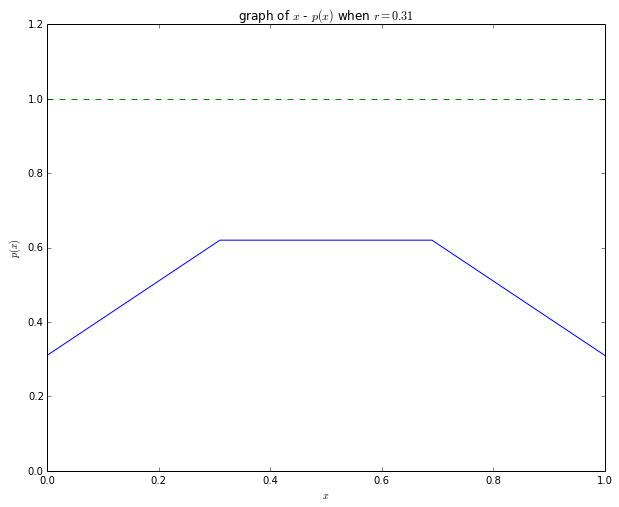
\includegraphics{output_23_0.png}

\(k+1\)番目の発言\(x_{k+1}\)がなされた時、\(k\)番目までの発言のうち\(y\)個の発言が領域\([\max(0,x-r), \min(x+r,1)]\)の中に存在する確率は、
\begin{gather}
\begin{split}_{k}C_{y}p(r)^{y}p(r)^{k-y}\end{split}\notag
\end{gather}
で表せる。ここで注意すべき点は、\(p(x_{k}, r)\)は\(x_{k}\)によって変わるものであったから、\(x\)に対して期待値を取ったものを考えなければならないことである。\(p(r)\)はそのようにして得られた期待値であることを意味している。

すなわち\(p(r)\)は、

\(0<r\le0.5\)のとき
\begin{gather}
\begin{split}\begin{align}p(r) = E(p(x, r)) &= \int^{r}_{0}x+r\mathrm{d}x + \int^{1-r}_{r}2r \mathrm{d}x + \int^{1}_{1-r} 1-x+r \mathrm{d}x\\
&= \left[\frac{x^{2}}{2} + rx \right]^{r}_{0} + \left[ 2rx\right]^{1-r}_{r}+ \left[ x-\frac{x^{2}}{2} + rx\right]^{1}_{1-r}\\
&= -r^{2} + 2r \end{align}\end{split}\notag
\end{gather}
\(0.5<r\le1\)のときも同様にして
\begin{gather}
\begin{split}p(r) = E(p(x,r)) = -r^{2} + 2r\end{split}\notag
\end{gather}
である。

また、式()は
\begin{gather}
\begin{split}P[X=y] =\ _{k}C_{y}p(r)^{y}(1-p(r))^{k-y}\end{split}\notag
\end{gather}
のように書けば明らかなように、確率変数\(X\)に対するパラメータ\(k,p\)の二項分布\(B(k,p)\)を表している。

この時、確率変数\(X\)に対する期待値と分散は、
\begin{gather}
\begin{split}E(X) = kp(r)\end{split}\notag
\end{gather}\begin{gather}
\begin{split}V(X) = kp(r)(1-p(r))\end{split}\notag
\end{gather}
である。

時刻\(k\)が大きい時、具体的には
\begin{gather}
\begin{split}kp(r) > 5,\end{split}\notag
\end{gather}\begin{gather}
\begin{split}kp(r)(1-p(r)) > 5\end{split}\notag
\end{gather}
をみたす\(k\)のとき、二項分布は正規分布に近似できるので、期待値は中央値とほぼ等しくなる。すなわち、\(y=kp(r)\)より多くの点を見出す確率\(P[X\le y]\)は、どんな時刻\(k\)においても\(1/2\)となる。

すなわち、時刻の依存性はないため、\(x_{k+1}\)のまわりの領域に\(y\)個以上の他の点が存在する場合を1、存在しない場合を0とすれば、これらの起こる確率は、それぞれ\(1/2\)であり、\(k\)回目に\(y\)個以上のエッジが張られて試行が終了する確率は、\(p=1/2\)の\href{http://ja.wikipedia.org/wiki/\%E5\%B9\%BE\%E4\%BD\%95\%E5\%88\%86\%E5\%B8\%83}{幾何分布}に従う:
\begin{gather}
\begin{split}P[X=k] = \left( \frac{1}{2} \right)^{k}\end{split}\notag
\end{gather}
このときの期待値と分散は
\begin{gather}
\begin{split}E(X) = \frac{1}{p} = 2\end{split}\notag
\end{gather}\begin{gather}
\begin{split}V(X) = \frac{1-p}{p^{2}} = 2\end{split}\notag
\end{gather}
すなわち、これまでのような場合を考えたとすると、平均として2回で試行が終了し、ほとんどの試行は1\textasciitilde{}3回で終了することになる。しかし、これは先程述べたような二項分布の正規分布への近似ができない領域であることに注意が必要である。したがって、実際には\(y\)の選び方をうまく選ぶことによって(たとえば試行が終了する回数の期待値が、二項分布を正規分布に近似できるような\(k\)となるように\(p\)を決めるような\(y\))、実際に\(k\)の期待値はこの確率分布のものと等しくなるだろう。


\section{1-B. 参加者を距離で決まる確率で選び、その中から意見が一様に選ばれる場合}
\label{draft:b}
次に考えるのは、自然な例として、発言者間の距離が定義されているようなものを考える。ここで言う''距離''とは、実際の発言者間の物理的な距離だけでなく、それぞれの間の関係性や声の大きさなどの概念を内包したものと考えることもできるだろう。実際には、そのように距離の計算に用いるパラメータが\(b\)個あるとして、そのパラメータを要素とする元とそれからなる空間に対して距離を考える。

簡単な例として\(b\)次元ユークリッド距離を取ることを考える。すなわち\(b\)個のパラメータを要素とする元からなる空間\(X\)があった時、

距離関数\(d: X \times X \rightarrow \mathbb{R}\)が
\begin{gather}
\begin{split}d(x, y) = \sqrt{\sum_{i=1}^{b}(x_{i}-y_{i})^{2}}\ \ ,\ x,y\in X\end{split}\notag
\end{gather}
と書けることを意味する。実際の場合には、各データ同士の相関を考慮に入れたマハラノビス距離などのほうが適当な場合もあるかもしれないが、まずはイメージしやすいということでユークリッド距離を考えた。

以下では、記述の簡単にするため、人\(i\)と人\(j\)の間の距離を\(d_{ij}\)と書くことにする。

時刻\(k\)に\(i\)が発言を行い、その後時刻\(k+1\)に\(j\)が発言\(x_{k+1}^{j}\)を行う確率\(p_{k}(i,j)\)は、距離\(d_{ij}\)の関数として、次のようにできる。
\begin{gather}
\begin{split}p_{k}(i,j) = \frac{g_{k}(d_{ij})}{\sum_{j} g_{k}(d_{ij})}\end{split}\notag
\end{gather}
この\(g\)の選び方によって、距離の大きさがどのように確率に重みを持たせるかということが決定される。一般に\(g\)は時刻\(k\)によって変化してもいいので、添字\(k\)をつけて時刻\(k\)における関数であることを表した。

単純な例として\(g_{k}(d) = const.,\ ^{\forall}k, d\in \mathbb{R}^{1}\)とすると、距離に依らず発言者が選ばれるわけなので、1-Aの発言者の選び方と同じである。

\(g(d)\)は\([0, +\infty]\)で定義される非負の実関数であればよい。

ex)
\begin{gather}
\begin{split}g(d) = \frac{1}{d+1}\end{split}\notag
\end{gather}\begin{gather}
\begin{split}g(d) = e^{-d}\end{split}\notag
\end{gather}\begin{gather}
\begin{split}g(d) = \left\{ \begin{array}{ll} c & (0\le d \le 1/c) \\
1/d & (d>1/c) \\
\end{array}\right., \ \ c>0\end{split}\notag
\end{gather}
しかし、ここで注意すべき点として、どの発言者が発言するにしても、1-Aで考えたように、どの発言者も\([0,1]\)の一様乱数を取るなら、結局、意見について見たときの試行は同様のことをしており、誰が発言したかは本質的な問題にはならないことが分かる。

これまでの設定を用いて数値シミュレーションを行った結果を以下に示す。シミュレーションでは、確率を決める距離の関数\(g(d)\)として
\begin{gather}
\begin{split}g(d) = e^{-d}\end{split}\notag
\end{gather}
を採用し、意見の次元\(a=2\)、参加者の数\(N=6\)と設定する。

プログラムを実行すると、GUIのウィンドウが表示され、その中の青い丸が人の位置を表している。位置をドラッグして変更した後にプログラムを開始すると、はじめに人1が発言をした場合の、会議の進行がシミュレートされる。それぞれの人が発言する確率は先の関数\(g\)にしたがい、その確率で選ばれた人が、一様な確率で\([0,1]\)の中から意見を出す。以後この繰り返しで会議が進行し、意見の数が100を超えるたときシミュレーションを終了する。シミュレーションの結果得られるのは、時刻\(k\)において、「誰が発言したか」、「誰から誰にエッジが張られたか」、「いくつのエッジが張られたか」、の値を記録したものと、終了時までの人ごとの発現頻度、エッジの数の累積などである。

以下に作成したプログラムを示す。

\begin{Verbatim}[commandchars=\\\{\}]
\PYGZpc{}matplotlib inline

from Tkinter import *
import matplotlib.pyplot as plt
import numpy as np
import collections
import operator

def accumulate(iterable, func=operator.add):
    \PYGZsq{}Return running totals\PYGZsq{}
    \PYGZsh{} accumulate([1,2,3,4,5]) \PYGZhy{}\PYGZhy{}\PYGZgt{} 1 3 6 10 15
    \PYGZsh{} accumulate([1,2,3,4,5], operator.mul) \PYGZhy{}\PYGZhy{}\PYGZgt{} 1 2 6 24 120
    it = iter(iterable)
    total = next(it)
    yield total
    for element in it:
        total = func(total, element)
        yield total


class Person(object):

    def \PYGZus{}\PYGZus{}init\PYGZus{}\PYGZus{}(self, ideas\PYGZus{}num=10, place=(0., 0.), **kwargs):
        \PYGZsh{} 意見は0\PYGZti{}1の間の値を一様に取りうる
        self.ideas = list(np.random.random(ideas\PYGZus{}num))
        \PYGZsh{} 発言者の実際の位置が2次元の座標として表せる
        self.place = place
        \PYGZsh{} その他の特徴量
        for (k, v) in kwargs.items():
            setattr(self, k, v)

    def distance(self, p):
        \PYGZsh{} 人pと自分との間の距離(ユークリッド距離)
        d = np.sqrt((self.place[0]\PYGZhy{}p.place[0])**2 + (self.place[1]\PYGZhy{}p.place[1])**2)
        return d


class meeting(object):

    def \PYGZus{}\PYGZus{}init\PYGZus{}\PYGZus{}(self, N):
        \PYGZsh{} 会議の参加人数
        self.N = N
        \PYGZsh{} 意見の時系列
        self.ideas = []
        \PYGZsh{} 発言者の時系列
        self.speaker = []
        \PYGZsh{} 時刻
        self.k = 0
        self.K = 100
        \PYGZsh{} 張られたリンク(時刻, 時刻)のタプルで表現する
        self.links = []
        \PYGZsh{} リンクの数(各時刻)
        self.l = [0]
        \PYGZsh{} リンクの数(累計)
        self.L = [0]

    def g(self, x):
        \PYGZsh{} 発言者の物理的距離に対する関数
        return np.exp(\PYGZhy{}x)

    def p(self, i):

        \PYGZsh{} 参加者の中で話せる人のみを対象に
        \PYGZus{}N = []
        for k in range(1, self.N+1):
            if len(self.members[k].ideas):
                \PYGZus{}N.append(k)

        \PYGZsh{} それらの人たちに対し、関数gによる重み付けの確率を付与
        w = []
        for n in \PYGZus{}N:
            d = self.members[n].distance(i)
            w.append(self.g(d))
        w = np.array(w)
        sum\PYGZus{} = np.sum(w)
        \PYGZus{}p = list(w/sum\PYGZus{})
        p = list(accumulate(\PYGZus{}p))
        rn = np.random.rand()
        nm = 0
        while True:
            if p[nm] \PYGZgt{} rn:
                break
            else:
                nm += 1
        \PYGZsh{} その確率で選ばれた人の名前を返す
        j = \PYGZus{}N[nm]
        return j

    def q(self, j):
        \PYGZsh{} 発言者jが選ばれた時、持っている意見から等確率で意見を取り出す
        x\PYGZus{}j = self.members[j]
        return np.random.rand()  \PYGZsh{}x\PYGZus{}j.ideas.pop()

    def distance(self, x, y):
        \PYGZsh{} 意見の近さを絶対値で表現
        d = np.abs(x \PYGZhy{} y)
        if d == 0:
            return self.radius + 1
        else:
            return d

    def connect(self):
        l = 0
        for i, v in enumerate(self.ideas[:\PYGZhy{}1]):
            \PYGZsh{} k番目の意見と意見が近い時、それらノードの間にリンクを形成する
            if self.distance(v, self.ideas[self.k]) \PYGZlt{} self.radius:
                self.links.append((i, self.k))
                l += 1
        return l

    def check\PYGZus{}agreement(self):
        \PYGZsh{} 合意チェック 参加人数Nによる関数
        def L(N):
            return N**2
        \PYGZsh{}if self.l[\PYGZhy{}1] \PYGZgt{} L(self.N):
        if self.k \PYGZgt{} self.K:
            return True
        else:
            return False

    def check\PYGZus{}ideas(self):
        for k in range(1, self.N+1):
            if len(self.members[k].ideas):
                return True
        return False

    def f\PYGZus{}L(self):
        \PYGZsh{} リンクから会議の評価
        \PYGZsh{} 単純に会議終了時に得られたリンクの数を返す
        return self.L[\PYGZhy{}1]

    def f\PYGZus{}T(self):
        \PYGZsh{} 会議に必要な時間の評価
        \PYGZsh{} 単純に必要な時間kを返す
        return self.k

    def f(self):
        \PYGZsh{} f\PYGZus{}Lとf\PYGZus{}Tを使った評価関数f
        return self.f\PYGZus{}L() \PYGZhy{} self.f\PYGZus{}T()

    def end(self):
        \PYGZsh{} 会議の通常終了、各定義量の計算や受け渡しなどはここで
        plt.ioff()
        plt.show()

        \PYGZsh{} ネットワーク図を描画
        link\PYGZus{}s = [(a, b) for a, b in zip(self.speaker[:\PYGZhy{}1], self.speaker[1:])]
        counter\PYGZus{}links = collections.Counter(link\PYGZus{}s)
        for link, lw in counter\PYGZus{}links.items():
            ix = self.members[link[0]].place[0]
            iy = self.members[link[0]].place[1]
            jx = self.members[link[1]].place[0]
            jy = self.members[link[1]].place[1]
            \PYGZus{}x, \PYGZus{}y = ((ix+jx)/2, (iy+jy)/2)
            if link[0] == link[1]:
                continue
            elif link[0] \PYGZlt{} link[1]:
                color = \PYGZsq{}black\PYGZsq{}
                va = \PYGZsq{}bottom\PYGZsq{}
            else:
                color = \PYGZsq{}red\PYGZsq{}
                va = \PYGZsq{}top\PYGZsq{}

            plt.plot([ix, jx], [iy, jy], color=color, lw=lw*4/self.k+1)
            plt.text(\PYGZus{}x, \PYGZus{}y, \PYGZsq{}(\PYGZpc{}d,\PYGZpc{}d)\PYGZsq{} \PYGZpc{} (link[0], link[1]),
                     color=color, va=va)

        counter = collections.Counter(self.speaker)

        for key, i in self.members.items():
            x = i.place[0]
            y = i.place[1]
            size = counter[key] * 30
            plt.scatter(x, y, s=size)
            plt.text(x, y, str(key), color=\PYGZsq{}green\PYGZsq{})
        plt.show()

        \PYGZsh{} 各時刻に追加されたリンク数のグラフ
        r = self.radius
        k = np.arange(self.k + 1)
        y = (\PYGZhy{}r**2 + 2*r)*k
        delta = np.sqrt((\PYGZhy{}r**4 + 4*r**3 \PYGZhy{} 5*r**2 + 2*r)*k)
        y1 = y + delta
        y2 = y \PYGZhy{} delta
        plt.fill\PYGZus{}between(k, y1, y2, facecolor=\PYGZsq{}green\PYGZsq{}, alpha=0.2)
        plt.plot(k, self.l)
        plt.plot(k, y)
        plt.xlabel(r\PYGZdq{}\PYGZdl{}k\PYGZdl{}\PYGZdq{})
        plt.ylabel(r\PYGZdq{}\PYGZdl{}l\PYGZdl{}\PYGZdq{})
        plt.show()

        \PYGZsh{} リンク数の累積グラフ
        plt.plot(k, self.L)
        plt.plot(k, (\PYGZhy{}self.radius**2 + 2*self.radius)*k**2/2.)
        plt.xlabel(r\PYGZdq{}\PYGZdl{}k\PYGZdl{}\PYGZdq{})
        plt.ylabel(r\PYGZdq{}\PYGZdl{}L\PYGZdl{}\PYGZdq{})
        plt.show()

        \PYGZsh{} 時系列で発言者の表示
        \PYGZsh{} print \PYGZsq{}self.speaker:\PYGZsq{}, self.speaker

        \PYGZsh{} 評価関数を通した結果
        \PYGZsh{} print \PYGZsq{}self.f\PYGZsq{}, self.f()

    def end2(self):
        \PYGZsh{} 会議の異常終了(発言者が発言できなくなる)
        pass

    def init(self):
        x = [i.place[0] for i in self.members.values()]
        y = [i.place[1] for i in self.members.values()]
        plt.scatter(x, y)
        plt.ion()
        plt.draw()

    def callback(self):
        \PYGZsh{} print \PYGZsq{}speaker:\PYGZsq{}, self.speaker[\PYGZhy{}1]
        \PYGZsh{} print \PYGZsq{}link:\PYGZsq{}, self.l[\PYGZhy{}1]
        ix = self.members[self.speaker[\PYGZhy{}2]].place[0]
        iy = self.members[self.speaker[\PYGZhy{}2]].place[1]
        jx = self.members[self.speaker[\PYGZhy{}1]].place[0]
        jy = self.members[self.speaker[\PYGZhy{}1]].place[1]
        plt.plot([ix, jx], [iy, jy])
        plt.text((ix+jx)/2, (iy+jy)/2, \PYGZsq{}\PYGZpc{}d:(\PYGZpc{}d,\PYGZpc{}d)\PYGZsq{}
                 \PYGZpc{} (self.k, self.speaker[\PYGZhy{}2], self.speaker[\PYGZhy{}1]))
        plt.draw()

    def progress(self):
        self.init()
        \PYGZsh{} はじめに1が発言するとする
        self.ideas.append(self.q(1))
        self.speaker.append(1)
        while True:
            j = self.p(self.members[self.speaker[\PYGZhy{}1]])
            self.ideas.append(self.q(j))
            self.speaker.append(j)
            self.k += 1
            self.l.append(self.connect())
            self.L.append(len(self.links))
            self.callback()
            if self.check\PYGZus{}agreement():
                print \PYGZdq{}\PYGZbs{}nnormal end\PYGZdq{}
                self.end()
                break
            if not self.check\PYGZus{}ideas():
                print \PYGZdq{}\PYGZbs{}nno one can speak\PYGZdq{}
                self.end2()
                break


class Main:

    def \PYGZus{}\PYGZus{}init\PYGZus{}\PYGZus{}(self, radius=0.3):
        N = 6
        self.app = meeting(N)
        self.app.radius = radius
        window = Window(N, main=self.app)
        window.display()

class Window(object):

    def \PYGZus{}\PYGZus{}init\PYGZus{}\PYGZus{}(self, N, main):
        self.root = Tk()
        self.main = main
        self.width = 640
        self.height = 480
        self.canvas = Canvas(self.root, width=self.width, height=self.height)
        self.var = StringVar()
        self.oval(self.canvas, N)
        self.canvas.bind(\PYGZsq{}\PYGZlt{}Motion\PYGZgt{}\PYGZsq{}, self.pointer)
        self.canvas.pack()
        label = Label(self.root, textvariable=self.var, font=\PYGZsq{}Ubuntu 9\PYGZsq{})
        label.pack(side=\PYGZsq{}left\PYGZsq{})
        b1 = Button(self.root, text=\PYGZsq{}start\PYGZsq{}, command=self.b1\PYGZus{}clicked)
        b1.pack(side=\PYGZsq{}right\PYGZsq{})
        b2 = Button(self.root, text=\PYGZsq{}save\PYGZsq{}, command=self.b2\PYGZus{}clicked)
        b2.pack(side=\PYGZsq{}right\PYGZsq{})

    def oval(self, canvas, N=6):
        self.members = dict()
        deg = np.linspace(0., 360., N, endpoint=False)
        radius = 20
        self.r = int((min(self.height, self.width)/2\PYGZhy{}radius)*0.9)
        self.centerx = int(self.width/2)
        self.centery = int(self.height/2)
        for n in range(1, N+1):
            rad = np.radians(deg[n\PYGZhy{}1])
            self.members[n] = Oval(canvas, n,
                                   self.centerx+self.r*np.cos(rad),
                                   self.centery+self.r*np.sin(rad),
                                   radius, self.var)

    def pointer(self, event):
        self.var.set(\PYGZdq{}(\PYGZpc{}d,\PYGZpc{}d)\PYGZdq{} \PYGZpc{} (event.x, event.y))

    def b1\PYGZus{}clicked(self):
        self.main.members = dict()
        for n in range(1, self.main.N+1):
            x = (self.members[n].x\PYGZhy{}self.centerx)/float(self.r)
            y = (self.members[n].y\PYGZhy{}self.centery)/float(self.r)
            self.main.members[n] = Person(place=(x, y))
        self.main.progress()
        self.root.destroy()

    def b2\PYGZus{}clicked(self):
        import tkFileDialog
        import os

        fTyp = [(\PYGZsq{}eps file\PYGZsq{}, \PYGZsq{}*.eps\PYGZsq{}), (\PYGZsq{}all files\PYGZsq{}, \PYGZsq{}*\PYGZsq{})]
        filename = tkFileDialog.asksaveasfilename(filetypes=fTyp,
                                                  initialdir=os.getcwd(),
                                                  initialfile=\PYGZsq{}figure\PYGZus{}1.eps\PYGZsq{})

        if filename is None:
            return
        try:
            self.canvas.postscript(file=filename)
        except TclError:
            print \PYGZdq{}\PYGZdq{}\PYGZdq{}
            TclError: Cannot save the figure.
            Canvas Window must be alive for save.\PYGZdq{}\PYGZdq{}\PYGZdq{}
            return 1

    def display(self):
        self.root.mainloop()


class Oval:

    def \PYGZus{}\PYGZus{}init\PYGZus{}\PYGZus{}(self, canvas, id, x, y, r, var):
        self.c = canvas
        self.x = x
        self.y = y
        self.var = var
        self.tag = str(id)
        self.c.create\PYGZus{}oval(x\PYGZhy{}r, y\PYGZhy{}r, x+r, y+r, outline=\PYGZsq{}\PYGZsq{}, fill=\PYGZsq{}\PYGZsh{}069\PYGZsq{}, tags=self.tag)

        self.c.tag\PYGZus{}bind(self.tag, \PYGZsq{}\PYGZlt{}Button\PYGZhy{}1\PYGZgt{}\PYGZsq{}, self.pressed)
        self.c.tag\PYGZus{}bind(self.tag, \PYGZsq{}\PYGZlt{}Button1\PYGZhy{}Motion\PYGZgt{}\PYGZsq{}, self.dragging)

    def pressed(self, event):
        self.x = event.x
        self.y = event.y

    def dragging(self, event):
        self.c.move(self.tag, event.x \PYGZhy{} self.x, event.y \PYGZhy{} self.y)
        self.x = event.x
        self.y = event.y
\end{Verbatim}

\begin{Verbatim}[commandchars=\\\{\}]
\PYG{n}{main} \PYG{o}{=} \PYG{n}{Main}\PYG{p}{(}\PYG{n}{radius}\PYG{o}{=}\PYG{l+m+mf}{0.3}\PYG{p}{)}
\end{Verbatim}

\begin{Verbatim}[commandchars=\\\{\}]
normal end
\end{Verbatim}

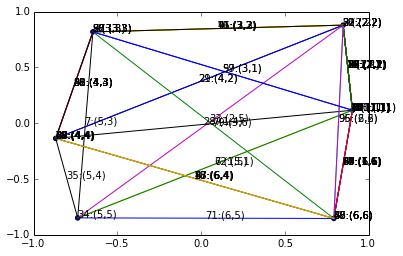
\includegraphics{output_39_1.png}

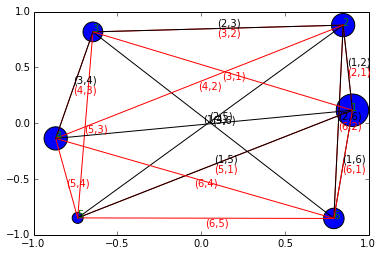
\includegraphics{output_39_2.png}

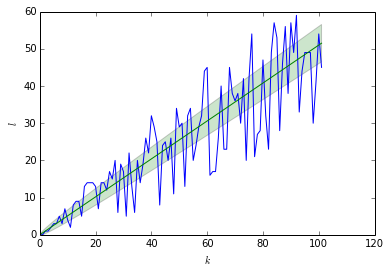
\includegraphics{output_39_3.png}

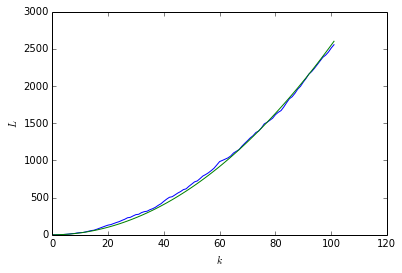
\includegraphics{output_39_4.png}

図1. 発言者の発現頻度とエッジのグラフ

図2. 時刻\(k\)に選ばれた点から張られたエッジの数

図3.時刻\(k\)までのエッジの数の総和

これらのグラフからも確かめられることだが、1-Aで考えたとおり、意見の近さに関する閾値\(r\)を定めて、その範囲に既になされた発言が存在するときにエッジを張るようにすると、時刻\(k\)にある点が選ばれたときに張られるエッジの数は、二項分布\(B(k, p)\)にしたがっていたので、その期待値は試行回数\(k\)に比例する(\(E(X) = kp(r)\))。

このときの傾きは、\(p(x, r)\)の\(x\)に関する期待値\(p(r)=-r^{2}+2r\)であるから、\(r\)に関してプロットすると以下のようになる。

図4.図2の緑の直線の傾きと\(r\)の間の関係

上図の場合、\(r\)に対応する値として\code{self.radius=1/.3}としているので、傾きの平均値は\(-1/3(1/3-2) = 5/9\)である(緑の線)。また、累積のリンク数についても、同じように曲線でフィットすることができている。


\section{2. 過去の意見を参照にして次の意見を決める場合}
\label{draft:id6}
1の場合には、人を選ぶ確率とそのうえで意見が選ばれる確率は独立であるというものであった。しかし、これまで考えたように、単にそのようなモデルを考えただけだと人数の効果をうまく反映できないように思える。したがって、次に考えるモデルは、人がそれぞれ意見をもっており、前の発言に関して意見が近い、または反対意見を持っている時にはその意見をもつ人が発言する確率が高い、というようなものを考える。

アルゴリズムとしては、はじめに参加者たち\(P=\{i\ |\ i = 0, 1, 2,\cdots , n-1\}\)はそれぞれに独自の\(s_{i}\)個の意見を持っているとする。このときの意見\(X\)は状態空間\(S\)上のある一点を指しており、ベクトルで記述されるようなものである。意見すべての集合は互いに重なりあうことはなく(全く同じ点に異なる人の意見が存在することはない。)、それぞれが異なる分布を持っていてもよい。はじめに議題、すなわち時刻\(0\)における意見が作られ、次に時刻1では、それぞれの参加者の意見のうちから、一番その意見によって発言されやすいものをそれぞれ一つずつ選ぶ。これを大きい順に並べ替えて、一番発言しやすい人から順に発言の機会が与えられる。それぞれの人には発言力\(P_{i}\)が割り当てられており、その値によって確率的に発言するかどうかが決まる。すなわち、意見の近さが試行の順番を決め、自分の番が回ってきたときに発言するかどうかの確率は一定であるという場面を考えている。

別の方法としては、この発言力と意見のしやすさを合わせた指標で発言するかどうかを決めるという方法があるが、まずは簡単のために、はじめにそれぞれが自分の中で一番近い意見を持ち寄り、その順番に発言の権利が与えられていくような場面を考えることにする。また、最終的に誰も発言できない場合もあるので、そのときには沈黙があったとして時間は1進めて同じ意見について先ほどまでと同じ試行を繰り返すこととする。


\section{2-A. 過去の意見の影響を受けない場合}
\label{draft:id7}
全部で\(n\)人のなかで人\(i\)が\(r+1\)(\(r = 1, 2, \cdots , n-1\))番目に発言する権利を得たとき、自分まで発言権が回ってくる確率は、
\begin{gather}
\begin{split}p_{r+1}(i) = \frac{\sum_{J = <j_{0}, \cdots ,j_{r-1}>_{r}}\prod_{j\in J}(1-P_{j})}{_{n-1}C_{r}}\end{split}\notag
\end{gather}
ここで\(J = <j_{0}, j_{1}, \cdots ,j_{r-1}>_{r}\)は、\(i\)を除く\(n-1\)個の要素から\(r\)個取り出す組み合わせのうちの1揃いをあらわすことにす
る。

また、1番目に発言する権利を得たときは、発言権が回ってくる確率は当然
\begin{gather}
\begin{split}p_{0}(i) = 1\end{split}\notag
\end{gather}
である。

具体例として以下のようなものを考える。

\(N=\{0,1,2,3,4\}, n = 5, i = 1, r = 2\)とすると、人1までに2人いるはずであり、その2人についての組み合わせは\((0,2), (0,3), (0,4), (2,3), (2,4), (3,4)\)の6つの組み合わせがある。上の式では\(J\)の一つは\((0, 2)\)であり、このとき\(j_{0} = 0, j_{1} = 2\)である。この\(J\)に関して和をとり、組み合わせの数\(\ _{4}C_{2} = 6\)で割って期待値を求めている。
\begin{gather}
\begin{split}\begin{align}
p_{r+1}(1) &= \left[(1-P_{0})(1-P_{2}) + (1-P_{0})(1-P_{3}) + (1-P_{0})(1-P_{4}) \right.\\
&\ \left. + (1-P_{2})(1-P_{3}) + (1-P_{2})(1-P_{4}) + (1-P_{3})(1-P_{4}) \right]/6
\end{align}\end{split}\notag
\end{gather}
人\(i\)が発言権の順番で\(r\)番目になる確率は等しいので、\(r\)に関する平均をとり、\(P_{i}\)をかければ、これは人\(i\)が発言する確率の期待値となる。
\begin{gather}
\begin{split}p(i) = \frac{\sum_{r=0}^{n}p_{r}(i)P_{i}}{n}.\end{split}\notag
\end{gather}
このとき得られた確率は人\(i\)によって異なり、期待値としては毎時刻ごとにそれぞれの人がその確率で発言することになり、単純な確率過程に帰着できる。


\section{2-B. 1つ前の意見を参照する場合}
\label{draft:b-1}
それぞれの人が同じ確率\(p\)で自分の番が来たときに発言するとしたとき、議題、すなわちはじめに与えられた意見のみを参照する場合と、一つ前の意見のみを参照する場合の二つの場合に関してシミュレーションを行った。このシミュレーションでは、先に述べたように各参加者の意見のうち、参照する意見に一番近いものを選び、その意見の近さの順に確率\(p\)でその意見を選ぶかどうかを決めている。このときに得られた意見のネットワークを実際の2次元の意見空間上に表したものを以下に示す。

作成したプログラムを以下に示す。

\begin{Verbatim}[commandchars=\\\{\}]
\PYGZpc{}matplotlib inline
import numpy as np
from scipy.spatial.distance import euclidean as euc
import matplotlib.pyplot as plt
import mpld3
from mpld3 import plugins
from mpld3.utils import get\PYGZus{}id


class Person:

    def \PYGZus{}\PYGZus{}init\PYGZus{}\PYGZus{}(self, S, a, p=0.5):
        self.S = S
        self.a = a
        self.p = p

    def gather(self):
        \PYGZdq{}\PYGZdq{}\PYGZdq{}make person to participate the meeting.
        \PYGZdq{}\PYGZdq{}\PYGZdq{}
        self.ideas = self.has\PYGZus{}idea()

    def has\PYGZus{}idea(self):
        \PYGZdq{}\PYGZdq{}\PYGZdq{}a person has self.S ideas with self.a dimension.
        \PYGZdq{}\PYGZdq{}\PYGZdq{}
        return list(np.random.rand(self.S, self.a))

    def chose\PYGZus{}idea(self, idea, idea2=None):
        alpha = 2.5
        beta = 1.
        if len(self.ideas) == 0:
            return False
        \PYGZsh{} return min(d) and its idea\PYGZus{}id
        if idea2 == None:
            return min([(euc(vec, idea), idea\PYGZus{}id) for idea\PYGZus{}id, vec in enumerate(self.ideas)])
        else:
            return min([(alpha*euc(vec, idea) + beta*euc(vec, idea2), idea\PYGZus{}id)
                        for idea\PYGZus{}id, vec in enumerate(self.ideas)])

class Meeting:

    \PYGZdq{}\PYGZdq{}\PYGZdq{}Simulate a meeting with \PYGZdq{}simple3\PYGZdq{} situation.

    Give keyword arguments:

        K = 20 \PYGZsh{} Time limit
        N = 6 \PYGZsh{} a number of participants
        S = 10 \PYGZsh{} a number of ideas for each participants
        a = 2 \PYGZsh{} the dimension of an idea
        p = 0.5 \PYGZsh{} probability that a person speak
        draw = True \PYGZsh{} draw image or don\PYGZsq{}t

    Output:

        self.minutes: list of
                      ( idea(which is vector with a dimension)
                      , who(person\PYGZus{}id in the list \PYGZdq{}self.membes\PYGZdq{}))
        self.k: stopped time (=len(self.minutes))
    \PYGZdq{}\PYGZdq{}\PYGZdq{}

    def \PYGZus{}\PYGZus{}init\PYGZus{}\PYGZus{}(self, K=20, N=6, S=10, a=2, p=0.5, draw=True, case=2):
        self.K = K
        self.N = N
        self.S = S
        self.a = a
        self.p = p
        self.draw = draw
        self.case = case  \PYGZsh{} case in the above cell: 2, 3, 4 or 5
        if not self.case in [2, 3, 4, 5]:
            raise ValueError
        self.members = []
        self.minutes = []  \PYGZsh{} list of (idea, who)
        self.k = 0

    def gather\PYGZus{}people(self):
        \PYGZdq{}\PYGZdq{}\PYGZdq{}gather people for the meeting.

        You can edit what ideas they have in here.
        \PYGZdq{}\PYGZdq{}\PYGZdq{}
        for n in range(self.N):
            person = Person(self.S, self.a, self.p)
            \PYGZsh{} person.has\PYGZus{}idea = some\PYGZus{}function()
            \PYGZsh{} some\PYGZus{}function: return list of self.S arrays with dim self.a.
            person.gather()
            self.members.append(person)

    def progress(self):
        \PYGZdq{}\PYGZdq{}\PYGZdq{}meeting progress
        \PYGZdq{}\PYGZdq{}\PYGZdq{}
        self.init()
        preidea = self.subject
        prepreidea = None
        self.k = 1

        while self.k \PYGZlt{} self.K + 1:
            \PYGZsh{} l: (distance, speaker, idea\PYGZus{}id) list for who can speak
            l = []
            for person\PYGZus{}id, person in enumerate(self.members):
                \PYGZsh{} chosed: (distance, idea\PYGZus{}id)
                chosed = person.chose\PYGZus{}idea(preidea, prepreidea)
                if chosed:
                    l.append((chosed[0], person\PYGZus{}id, chosed[1]))
            \PYGZsh{} if no one can speak: meeting ends.
            if len(l) == 0:
                print \PYGZdq{}no one can speak.\PYGZdq{}
                break
            i = [(person\PYGZus{}id, idea\PYGZus{}id)
                 for distance, person\PYGZus{}id, idea\PYGZus{}id in sorted(l)]

            for person\PYGZus{}id, idea\PYGZus{}id in i:
                rn = np.random.rand()
                if rn \PYGZlt{} self.members[person\PYGZus{}id].p:
                    idea = self.members[person\PYGZus{}id].ideas.pop(idea\PYGZus{}id)
                    self.minutes.append((idea, person\PYGZus{}id))
                    if self.case == 3:
                        preidea = idea
                    elif self.case == 4:
                        prepreidea = idea
                    elif self.case == 5:
                        prepreidea = preidea
                        preidea = idea
                    self.callback()
                    self.k += 1
                    break
            else:
                self.minutes.append((self.subject, self.N))
                self.callback()
                self.k += 1

        self.after()

    def init(self):
        self.gather\PYGZus{}people()
        self.subject = np.random.rand(self.a)
        self.minutes.append((self.subject, self.N))
        if self.draw:
            self.fig = plt.figure(figsize=(9, 9))
            self.ax = self.fig.add\PYGZus{}subplot(1, 1, 1)
            self.labels = [\PYGZsq{}subject\PYGZsq{}]
            self.s1 = [self.ax.scatter(self.subject[0], self.subject[1],
                                       c=next(self.ax.\PYGZus{}get\PYGZus{}lines.color\PYGZus{}cycle))]
            self.ax.text(
                self.subject[0], self.subject[1], \PYGZsq{}0\PYGZsq{}, fontsize=5)
            for i, member in enumerate(self.members):
                x = [vec[0] for vec in member.ideas]
                y = [vec[1] for vec in member.ideas]
                s = self.ax.scatter(
                    x, y, c=next(self.ax.\PYGZus{}get\PYGZus{}lines.color\PYGZus{}cycle), alpha=0.2)
                self.labels.append(str(i))
                self.s1.append(s)

    def callback(self):
        if self.draw:
            if self.minutes[\PYGZhy{}1][1] == self.N or self.minutes[\PYGZhy{}2][1] == self.N:
                alpha = 0.2
            else:
                alpha = 1.0
            ix = self.minutes[\PYGZhy{}2][0][0]
            iy = self.minutes[\PYGZhy{}2][0][1]
            jx = self.minutes[\PYGZhy{}1][0][0]
            jy = self.minutes[\PYGZhy{}1][0][1]
            l1 = self.ax.plot([ix, jx], [iy, jy], color=\PYGZsq{}black\PYGZsq{}, alpha=alpha)
            self.ax.text(jx, jy, \PYGZsq{}\PYGZpc{}d\PYGZsq{} \PYGZpc{} self.k, color=\PYGZsq{}blue\PYGZsq{}, fontsize=12)
        else:
            pass

    def after(self):
        if self.draw:
            plugins.connect(
                self.fig, plugins.InteractiveLegendPlugin(
                    self.s1, self.labels, ax=self.ax))
            mpld3.enable\PYGZus{}notebook()
        else:
            pass
\end{Verbatim}

\begin{Verbatim}[commandchars=\\\{\}]
\PYG{n}{meeting} \PYG{o}{=} \PYG{n}{Meeting}\PYG{p}{(}\PYG{n}{K}\PYG{o}{=}\PYG{l+m+mi}{30}\PYG{p}{,} \PYG{n}{N}\PYG{o}{=}\PYG{l+m+mi}{6}\PYG{p}{,} \PYG{n}{S}\PYG{o}{=}\PYG{l+m+mi}{50}\PYG{p}{,} \PYG{n}{a}\PYG{o}{=}\PYG{l+m+mi}{2}\PYG{p}{,} \PYG{n}{p}\PYG{o}{=}\PYG{l+m+mf}{0.6}\PYG{p}{,} \PYG{n}{case}\PYG{o}{=}\PYG{l+m+mi}{2}\PYG{p}{)}
\PYG{n}{meeting}\PYG{o}{.}\PYG{n}{progress}\PYG{p}{(}\PYG{p}{)}
\end{Verbatim}

\begin{Verbatim}[commandchars=\\\{\}]
\PYG{n}{meeting} \PYG{o}{=} \PYG{n}{Meeting}\PYG{p}{(}\PYG{n}{K}\PYG{o}{=}\PYG{l+m+mi}{30}\PYG{p}{,} \PYG{n}{N}\PYG{o}{=}\PYG{l+m+mi}{6}\PYG{p}{,} \PYG{n}{S}\PYG{o}{=}\PYG{l+m+mi}{50}\PYG{p}{,} \PYG{n}{a}\PYG{o}{=}\PYG{l+m+mi}{2}\PYG{p}{,} \PYG{n}{p}\PYG{o}{=}\PYG{l+m+mf}{0.6}\PYG{p}{,} \PYG{n}{case}\PYG{o}{=}\PYG{l+m+mi}{3}\PYG{p}{)}
\PYG{n}{meeting}\PYG{o}{.}\PYG{n}{progress}\PYG{p}{(}\PYG{p}{)}
\end{Verbatim}

これらの図から分かるように、一人辺りにもつ意見の数\(S\)を大きくすると、意見の密度を増加させるため、発言された意見の描く軌跡の範囲は小さくなる。

\(K=30, N=6, S=50, a=2, p=0.6\)のとき

2-B-a. 議題のみを参照

2-B-b. 一つ前の意見を参照

また、参加者の人数\(N\)を変えたときの平均頂点間距離の関係もグラフにし、以下に示すことにする。

一人あたりの意見の数\(S=50\)、意見の次元\(a=2\)、シミュレーションに用いた時系列\(K=30\)、自分に発言権が回ってきたときに発言する確率は、人に依らず\(p=0.6\)としたときの平均の意見間の距離を示すことにする。また、それぞれの\(N\)に対して100回の試行を平均したものをプロットに用いている。また、上段は通常のプロットであり、下段は両対数グラフとなっている。

図: 意見間の平均距離(ケース2)

図: 意見間の平均距離(ケース3)

また、参加者に発言の権利が回ってきたときに発言する確率\(p\)と、意見間の平均の距離との間の関係を見ることにする。例えばケース3(一つ前の意見からの近さで次の意見を選ぶモデル)のときに、会議の発言数\(K=30\)、人の数\(N=6\)、一人あたりの意見の数\(S=50\)としたときの\(p\)を変化させたときのグラフを示すことにする。

図:
発言者に発言権があるときに発言する確率\(p\)と意見間の平均距離との関係


\section{2-C. 2つの意見を参照する場合}
\label{draft:c-2}
次に、2つの意見を参照して次の意見を選ぶ場合を考えてみることにする。このときの意見の選ばれ方は、2-B-1,2-B-bの場合と同じく、意見の\(a\)次元ユークリッド距離の近さによって決める。しかしながら、参照とする点が2つあるために、この二つの点からの距離として適当なものを考える必要がある。2つの離れた場所に釘を刺し、一本のひもの両端をそれぞれの釘に結びつけて、ひもをピンと張った状態で円を書くようにすると、この二つの点を焦点とした楕円を書くことができる。この楕円の周上の点は同じ近さにあると考えて、2つの点から1つの点までの近さというものを評価することができる。したがって、2点\((y,z)\)からの点\(x\)までの近さの指標として、次のようなものが考えられる。ここで\(d(x,y)\)は通常の\(a\)次元ユークリッド距離であるとする。
\begin{gather}
\begin{split}D(x,(y,z)) = d(x,y) + d(x,z)\end{split}\notag
\end{gather}
また、この2つの意見との間のそれぞれの距離に関して重みをつけたものを考えることも出来る。すなわち、2つ前の意見に影響されるとはいえ、直前の意見ほどは影響されない、であるとか、一つ前の意見に影響されるとはいえ議題ほどには影響を受けない、などの条件を付加できるように
\begin{gather}
\begin{split}D(x,(y,z)) = \alpha d(x,y) + \beta d(x,z)\ \ (\alpha, \beta > 0)\end{split}\notag
\end{gather}
のように書くこともできる。

シミュレーションとしては行わないが、3つの意見を参照する場合、4つ、5つ・・・と、既に出ている意見の数まで参照点を増やすことができるので、一般には
\begin{gather}
\begin{split}D(x_{k+1}, (x_{1}, x_{2}, \cdots , x_{k})) = \sum_{i=1}^{k}w_{i}d(x_{k+1},x_{i})\ \ (w_{i} > 0)\end{split}\notag
\end{gather}
とできる。

また、別の近さの指標として、ベクトル\(\vec{Y}=y-x, \vec{Z} = z-x\)として、
\begin{gather}
\begin{split}D(x, (y,z)) \equiv | t \vec{Y} + (1-t)\vec{Z}|\ \ (0 \le t \le 1)\end{split}\notag
\end{gather}
とする方法もある。このとき、右辺の括弧の内部があらわすベクトルは、点\(y\),\(z\)を結んだ線分\(YZ\)を\((1-t):t\)に内分する点のベクトルを示しており、\(D\)はその点からのユークリッド距離をあらわすことになる。

このシミュレーションでは、先ほどの1つの意見を参照する場合に加えて、もう1つの意見の情報を保持しておくことにする。また、関数\code{find\_nearesr}で最も近い意見を探索するときの参照する点を2つにし、また、その時評価に用いる関数として上にあげた2つの近さの指標を用いることが出来るようにしてある。議題+1つ前の意見を参照する場合と、2つ前までの意見を参照する場合の2つの場合について、パラメータを変更しながらいくつかシミュレーションを行った。以下に示す図はその中の一例である。

\begin{Verbatim}[commandchars=\\\{\}]
\PYG{n}{meeting} \PYG{o}{=} \PYG{n}{Meeting}\PYG{p}{(}\PYG{n}{K}\PYG{o}{=}\PYG{l+m+mi}{30}\PYG{p}{,} \PYG{n}{N}\PYG{o}{=}\PYG{l+m+mi}{6}\PYG{p}{,} \PYG{n}{S}\PYG{o}{=}\PYG{l+m+mi}{50}\PYG{p}{,} \PYG{n}{a}\PYG{o}{=}\PYG{l+m+mi}{2}\PYG{p}{,} \PYG{n}{p}\PYG{o}{=}\PYG{l+m+mf}{0.6}\PYG{p}{,} \PYG{n}{case}\PYG{o}{=}\PYG{l+m+mi}{4}\PYG{p}{)}
\PYG{n}{meeting}\PYG{o}{.}\PYG{n}{progress}\PYG{p}{(}\PYG{p}{)}
\end{Verbatim}

\begin{Verbatim}[commandchars=\\\{\}]
\PYG{n}{meeting} \PYG{o}{=} \PYG{n}{Meeting}\PYG{p}{(}\PYG{n}{K}\PYG{o}{=}\PYG{l+m+mi}{30}\PYG{p}{,} \PYG{n}{N}\PYG{o}{=}\PYG{l+m+mi}{6}\PYG{p}{,} \PYG{n}{S}\PYG{o}{=}\PYG{l+m+mi}{50}\PYG{p}{,} \PYG{n}{a}\PYG{o}{=}\PYG{l+m+mi}{2}\PYG{p}{,} \PYG{n}{p}\PYG{o}{=}\PYG{l+m+mf}{0.6}\PYG{p}{,} \PYG{n}{case}\PYG{o}{=}\PYG{l+m+mi}{5}\PYG{p}{)}
\PYG{n}{meeting}\PYG{o}{.}\PYG{n}{progress}\PYG{p}{(}\PYG{p}{)}
\end{Verbatim}

\(K=30, N=6, S=50, a=2, p=0.6, \alpha=2.5, \beta=1\)のとき

2-C-a. 議題+一つ前の意見を参照

2-C-b. 二つ前までの意見を参照

2-C-bの結果については、2-B-bの場合、すなわち1つ前の意見を参照して次の意見を選んでいく場合に比べると、戻りの効果が大きくなるため、得られる軌跡はギザギザしており、最終的に到達する距離は小さくなっている。
それ以外の、人数や一人あたりの意見の数などに対する依存性は、それぞれのルールに対してあまり違いは見受けられない。

また、この場合に関しても平均の意見間の距離を測り、100回の試行の平均値を得たものを以下に示すことにする。ルールのほかの条件は揃えてあり、\(\alpha=1\)、\(\beta=1\)として楕円による近さの指標を用いて計算を行ったものを示している。

ここまでで、とりあえず2つまでの意見を参照する場合を考えてきたが、近さの指標を導入する際にも述べたように、この参照点は、それまでの意見の総数すべてまだ拡張することが出来る。しかしながら、議題を参照するかどうかの条件の違い以外では、先程まで考えたモデルに大きな相違は見られなかったため、参照点を増やしていくことは、人数との関係を考察していく上で本質的であるとは言えないだろう。したがって、これらのルールの違いによる差は一旦考えないことにし、人数との間でどのようにこの得られた軌跡の解析を行うことが出来るか、という点に着目していきたいと思う。


\section{3. 近距離抑制効果}
\label{draft:id8}
このモデルでは、2で考えたモデルと同様に、意見のネットワークを先に考えて、参加者の差異を無視してもよいとした場合の会議の進行を考察していく。

このモデルの特徴的なところは、意見を選んでいく過程を開始する前に、近い位置にある意見同士をエッジで結んでいき、クラスターを形成することである。こうして得られたクラスター1つの中の意見は、皆似た意見であるため、一度その中のどれか1つの点が選ばれると、それ以後そのクラスターに属する点はすべて選ばれることはないとする。また、意見の選び方は、前の意見から一番近い点をもつクラスターの中から、それぞれの人の発言確率によって、1つの意見を選ぶことにする。したって、意見の集約の閾値\(r\)が大きい時には、クラスターの大きさは大きくなり、クラスターの数は小さくなる。このようなときには、発言力のある人が何度も発言を行うことになり、発言力の小さい人は、同じクラスター上に意見をもっているために、発言を行う確率は小さくなる。

このように、実際の会議や会話から着想を得たモデルではあるが、その他の系への拡張も可能であると考えている。というのは、このように\(r\)を決めてその中の強いものが(実質的に)生き残り、その範囲にある他の弱い点は選ばれない(すなわち死んでいく)というのは、森の中の木の植生分布にもにた議論がある。すなわち、最適な密度というものが(対象とする系それぞれに関して)決まっており、その密度で分布するようになるということである。これは密度の小さい方から大きくしていく方向へ考えれば密度効果とも言うことができるし、先ほどの森の木の場合でははじめに密度が大きい状態から、自己間引き効果によって、最適な密度へと収束していくような場合を考えていることになる。

したがって、これらの言葉を使えば、意見空間上に分布する意見も、近いもの同士は吸収するか、まとめられるなどして同じものと見なされ、その密度は小さくなる効果を持っているということができる。このことによって、意見の密度は小さくなり、その最適な密度になっている状態で会議は進行するとみなしていることになる。

上で述べたような設定のもとでシミュレーションを行うプログラムを作成した。

クラスターの作成時には、(特に\(r\)が小さいときに)効率よく近接点を探すことができるよう、はじめに領域を長さ\(l(>r)\)の正方形の部分に分割する。これをセルと読んでいる。それぞれの意見がどのセルに入っているかを記録し、近い意見を探す際には、自分の所属するセルと、その周囲8マスを含めた9つのセルの中にある意見のみ考えればよい。また、これは境界では異なる振る舞いを見せるために、uniq\_listとmin、maxを使って、境界での参照セルが正しく選ばれるようにした。このようにして閾値\(r\)の内部にある点が選ばれたあと、その情報は保持され、ラベルを1から順につけていく。このとき、エッジを張られた先の点が、0(すなわちラベル付けされていない点)以外であったときは、その情報を覚えておき、すべての近接点を選んだ後に一番小さいラベルを、これらの選ばれた点に付与する。また、このとき他のクラスターとの融合も起きることがあり、その場合は、そのクラスター番号をもつ点のクラスター番号をすべて新しいより小さいラベルに更新することによって、同一のクラスターに所属していることを示すことにする。はじめに選ばれる意見はランダムであり、次の意見の選び方は、前の意見に最も近い意見をもつクラスターから選ぶこととする。選ばれたクラスターの中から意見を選ぶ方法は、それぞれの参加者の発言力と、クラスター内にある意見の数によって重み付きの確率が決められ、その確率によて1つの意見が選ばれる。今回のシミュレーションでは、この発言力に関しては、人によって差異はないとした。

\begin{Verbatim}[commandchars=\\\{\}]
\PYG{k}{def} \PYG{n+nf}{uniq\PYGZus{}list}\PYG{p}{(}\PYG{n}{seq}\PYG{p}{)}\PYG{p}{:}
    \PYG{n}{seen} \PYG{o}{=} \PYG{n+nb}{set}\PYG{p}{(}\PYG{p}{)}
    \PYG{n}{seen\PYGZus{}add} \PYG{o}{=} \PYG{n}{seen}\PYG{o}{.}\PYG{n}{add}
    \PYG{k}{return} \PYG{p}{[}\PYG{n}{x} \PYG{k}{for} \PYG{n}{x} \PYG{o+ow}{in} \PYG{n}{seq} \PYG{k}{if} \PYG{n}{x} \PYG{o+ow}{not} \PYG{o+ow}{in} \PYG{n}{seen} \PYG{o+ow}{and} \PYG{o+ow}{not} \PYG{n}{seen\PYGZus{}add}\PYG{p}{(}\PYG{n}{x}\PYG{p}{)}\PYG{p}{]}

\PYG{k}{def} \PYG{n+nf}{accumulate}\PYG{p}{(}\PYG{n}{iterable}\PYG{p}{,} \PYG{n}{func}\PYG{o}{=}\PYG{n}{operator}\PYG{o}{.}\PYG{n}{add}\PYG{p}{)}\PYG{p}{:}
    \PYG{l+s+sd}{\PYGZdq{}\PYGZdq{}\PYGZdq{}Return running totals}

\PYG{l+s+sd}{    Usage:}
\PYG{l+s+sd}{    accumulate([1,2,3,4,5]) \PYGZhy{}\PYGZhy{}\PYGZgt{} 1 3 6 10 15}
\PYG{l+s+sd}{    accumulate([1,2,3,4,5], operator.mul) \PYGZhy{}\PYGZhy{}\PYGZgt{} 1 2 6 24 120}
\PYG{l+s+sd}{    \PYGZdq{}\PYGZdq{}\PYGZdq{}}
    \PYG{n}{it} \PYG{o}{=} \PYG{n+nb}{iter}\PYG{p}{(}\PYG{n}{iterable}\PYG{p}{)}
    \PYG{n}{total} \PYG{o}{=} \PYG{n+nb}{next}\PYG{p}{(}\PYG{n}{it}\PYG{p}{)}
    \PYG{k}{yield} \PYG{n}{total}
    \PYG{k}{for} \PYG{n}{element} \PYG{o+ow}{in} \PYG{n}{it}\PYG{p}{:}
        \PYG{n}{total} \PYG{o}{=} \PYG{n}{func}\PYG{p}{(}\PYG{n}{total}\PYG{p}{,} \PYG{n}{element}\PYG{p}{)}
        \PYG{k}{yield} \PYG{n}{total}

\PYG{k}{def} \PYG{n+nf}{weighted\PYGZus{}choice}\PYG{p}{(}\PYG{n}{d}\PYG{p}{)}\PYG{p}{:}
    \PYG{n}{choices}\PYG{p}{,} \PYG{n}{weights} \PYG{o}{=} \PYG{n+nb}{zip}\PYG{p}{(}\PYG{o}{*}\PYG{n}{d}\PYG{p}{)}
    \PYG{n}{cumdist} \PYG{o}{=} \PYG{n+nb}{list}\PYG{p}{(}\PYG{n}{accumulate}\PYG{p}{(}\PYG{n}{weights}\PYG{p}{)}\PYG{p}{)}
    \PYG{n}{x} \PYG{o}{=} \PYG{n}{random}\PYG{o}{.}\PYG{n}{random}\PYG{p}{(}\PYG{p}{)} \PYG{o}{*} \PYG{n}{cumdist}\PYG{p}{[}\PYG{o}{\PYGZhy{}}\PYG{l+m+mi}{1}\PYG{p}{]}
    \PYG{k}{return} \PYG{n}{choices}\PYG{p}{[}\PYG{n}{bisect}\PYG{o}{.}\PYG{n}{bisect}\PYG{p}{(}\PYG{n}{cumdist}\PYG{p}{,} \PYG{n}{x}\PYG{p}{)}\PYG{p}{]}

\PYG{k}{class} \PYG{n+nc}{Person}\PYG{p}{:}

    \PYG{k}{def} \PYG{n+nf}{\PYGZus{}\PYGZus{}init\PYGZus{}\PYGZus{}}\PYG{p}{(}\PYG{n+nb+bp}{self}\PYG{p}{,} \PYG{n}{master}\PYG{p}{,} \PYG{n+nb}{id}\PYG{p}{,} \PYG{n}{ideas}\PYG{p}{,} \PYG{n}{w}\PYG{p}{)}\PYG{p}{:}
        \PYG{l+s+sd}{\PYGZdq{}\PYGZdq{}\PYGZdq{}Initialize argmunets.}

\PYG{l+s+sd}{        Keyword arguments:}
\PYG{l+s+sd}{        master    : Master class (call from \PYGZdq{}Meeting\PYGZdq{})}
\PYG{l+s+sd}{        self.id   : Id for each person [0, 1, ..., N\PYGZhy{}1]}
\PYG{l+s+sd}{        self.ideas: ideas in space [0,1] × [0,1]}
\PYG{l+s+sd}{        self.w    : probability weight for the person to speak}
\PYG{l+s+sd}{        \PYGZdq{}\PYGZdq{}\PYGZdq{}}
        \PYG{n+nb+bp}{self}\PYG{o}{.}\PYG{n}{id} \PYG{o}{=} \PYG{n+nb}{id}
        \PYG{n+nb+bp}{self}\PYG{o}{.}\PYG{n}{ideas} \PYG{o}{=} \PYG{n}{ideas}
        \PYG{n+nb+bp}{self}\PYG{o}{.}\PYG{n}{w} \PYG{o}{=} \PYG{n}{w}
        \PYG{c}{\PYGZsh{} add\PYGZus{}ideas : place, tag : (x, y), [person\PYGZus{}id, cluster\PYGZus{}id]}
        \PYG{n}{master}\PYG{o}{.}\PYG{n}{ideas} \PYG{o}{+}\PYG{o}{=} \PYG{p}{[}\PYG{p}{[}\PYG{p}{(}\PYG{n}{i1}\PYG{p}{,} \PYG{n}{i2}\PYG{p}{)}\PYG{p}{,} \PYG{p}{[}\PYG{n+nb+bp}{self}\PYG{o}{.}\PYG{n}{id}\PYG{p}{,} \PYG{l+m+mi}{0}\PYG{p}{,} \PYG{n+nb+bp}{self}\PYG{o}{.}\PYG{n}{w}\PYG{p}{]}\PYG{p}{]} \PYG{k}{for} \PYG{n}{i1}\PYG{p}{,} \PYG{n}{i2} \PYG{o+ow}{in} \PYG{n+nb+bp}{self}\PYG{o}{.}\PYG{n}{ideas}\PYG{p}{]}


\PYG{k}{class} \PYG{n+nc}{Cluster}\PYG{p}{:}

    \PYG{k}{def} \PYG{n+nf}{\PYGZus{}\PYGZus{}init\PYGZus{}\PYGZus{}}\PYG{p}{(}\PYG{n+nb+bp}{self}\PYG{p}{,} \PYG{n}{ideas}\PYG{p}{,} \PYG{n}{r}\PYG{p}{)}\PYG{p}{:}
        \PYG{l+s+sd}{\PYGZdq{}\PYGZdq{}\PYGZdq{}make cluster with self.r}

\PYG{l+s+sd}{        cluster\PYGZus{}link:}
\PYG{l+s+sd}{        \PYGZdq{}\PYGZdq{}\PYGZdq{}}
        \PYG{n+nb+bp}{self}\PYG{o}{.}\PYG{n}{ideas} \PYG{o}{=} \PYG{n}{ideas}
        \PYG{n+nb+bp}{self}\PYG{o}{.}\PYG{n}{r} \PYG{o}{=} \PYG{n}{r}
        \PYG{n+nb+bp}{self}\PYG{o}{.}\PYG{n}{l} \PYG{o}{=} \PYG{l+m+mi}{0}
        \PYG{n+nb+bp}{self}\PYG{o}{.}\PYG{n}{cluster\PYGZus{}link} \PYG{o}{=} \PYG{p}{[}\PYG{p}{]}
        \PYG{n+nb+bp}{self}\PYG{o}{.}\PYG{n}{clustering}\PYG{p}{(}\PYG{p}{)}

    \PYG{k}{def} \PYG{n+nf}{clustering}\PYG{p}{(}\PYG{n+nb+bp}{self}\PYG{p}{)}\PYG{p}{:}
        \PYG{n+nb+bp}{self}\PYG{o}{.}\PYG{n}{cell\PYGZus{}num} \PYG{o}{=} \PYG{n+nb}{int}\PYG{p}{(}\PYG{l+m+mf}{1.}\PYG{o}{/}\PYG{n+nb+bp}{self}\PYG{o}{.}\PYG{n}{r}\PYG{p}{)}
        \PYG{n}{lr} \PYG{o}{=} \PYG{l+m+mf}{1.}\PYG{o}{/}\PYG{n+nb+bp}{self}\PYG{o}{.}\PYG{n}{cell\PYGZus{}num}

        \PYG{n+nb+bp}{self}\PYG{o}{.}\PYG{n}{cell} \PYG{o}{=} \PYG{n+nb}{dict}\PYG{p}{(}\PYG{p}{)} \PYG{c}{\PYGZsh{} key: (cellx,celly), value: list of ids}
        \PYG{n+nb+bp}{self}\PYG{o}{.}\PYG{n}{rcell} \PYG{o}{=} \PYG{p}{[}\PYG{p}{]}
        \PYG{k}{for} \PYG{n}{i}\PYG{p}{,} \PYG{n}{idea} \PYG{o+ow}{in} \PYG{n+nb}{enumerate}\PYG{p}{(}\PYG{n+nb+bp}{self}\PYG{o}{.}\PYG{n}{ideas}\PYG{p}{)}\PYG{p}{:}
            \PYG{n}{cellx} \PYG{o}{=} \PYG{n+nb}{int}\PYG{p}{(}\PYG{n}{idea}\PYG{p}{[}\PYG{l+m+mi}{0}\PYG{p}{]}\PYG{p}{[}\PYG{l+m+mi}{0}\PYG{p}{]}\PYG{o}{/}\PYG{n}{lr}\PYG{p}{)}
            \PYG{n}{celly} \PYG{o}{=} \PYG{n+nb}{int}\PYG{p}{(}\PYG{n}{idea}\PYG{p}{[}\PYG{l+m+mi}{0}\PYG{p}{]}\PYG{p}{[}\PYG{l+m+mi}{1}\PYG{p}{]}\PYG{o}{/}\PYG{n}{lr}\PYG{p}{)}
            \PYG{k}{if} \PYG{n+nb+bp}{self}\PYG{o}{.}\PYG{n}{cell}\PYG{o}{.}\PYG{n}{has\PYGZus{}key}\PYG{p}{(}\PYG{p}{(}\PYG{n}{cellx}\PYG{p}{,} \PYG{n}{celly}\PYG{p}{)}\PYG{p}{)}\PYG{p}{:}
                \PYG{n+nb+bp}{self}\PYG{o}{.}\PYG{n}{cell}\PYG{p}{[}\PYG{p}{(}\PYG{n}{cellx}\PYG{p}{,} \PYG{n}{celly}\PYG{p}{)}\PYG{p}{]} \PYG{o}{+}\PYG{o}{=} \PYG{p}{[}\PYG{n}{i}\PYG{p}{]}
            \PYG{k}{else}\PYG{p}{:}
                \PYG{n+nb+bp}{self}\PYG{o}{.}\PYG{n}{cell}\PYG{p}{[}\PYG{p}{(}\PYG{n}{cellx}\PYG{p}{,} \PYG{n}{celly}\PYG{p}{)}\PYG{p}{]} \PYG{o}{=} \PYG{p}{[}\PYG{n}{i}\PYG{p}{]}
            \PYG{n+nb+bp}{self}\PYG{o}{.}\PYG{n}{rcell}\PYG{o}{.}\PYG{n}{append}\PYG{p}{(}\PYG{p}{(}\PYG{n}{cellx}\PYG{p}{,} \PYG{n}{celly}\PYG{p}{)}\PYG{p}{)}
        \PYG{n}{num} \PYG{o}{=} \PYG{l+m+mi}{1}
        \PYG{k}{for} \PYG{n}{i} \PYG{o+ow}{in} \PYG{n+nb}{range}\PYG{p}{(}\PYG{n+nb}{len}\PYG{p}{(}\PYG{n+nb+bp}{self}\PYG{o}{.}\PYG{n}{ideas}\PYG{p}{)}\PYG{p}{)}\PYG{p}{:}
            \PYG{n}{num} \PYG{o}{+}\PYG{o}{=} \PYG{n+nb+bp}{self}\PYG{o}{.}\PYG{n}{find\PYGZus{}nearest}\PYG{p}{(}\PYG{n}{i}\PYG{p}{,} \PYG{n}{num}\PYG{p}{)}
        \PYG{k}{return} \PYG{n+nb+bp}{self}\PYG{o}{.}\PYG{n}{cluster\PYGZus{}link}

    \PYG{k}{def} \PYG{n+nf}{find\PYGZus{}nearest}\PYG{p}{(}\PYG{n+nb+bp}{self}\PYG{p}{,} \PYG{n}{idea\PYGZus{}id}\PYG{p}{,} \PYG{n}{num}\PYG{p}{)}\PYG{p}{:}
        \PYG{l+s+sd}{\PYGZdq{}\PYGZdq{}\PYGZdq{}find nearest idea}

\PYG{l+s+sd}{        idea\PYGZus{}id: index in self.ideas}
\PYG{l+s+sd}{        \PYGZdq{}\PYGZdq{}\PYGZdq{}}
        \PYG{n}{cx}\PYG{p}{,} \PYG{n}{cy} \PYG{o}{=} \PYG{n+nb+bp}{self}\PYG{o}{.}\PYG{n}{rcell}\PYG{p}{[}\PYG{n}{idea\PYGZus{}id}\PYG{p}{]}
        \PYG{n}{place} \PYG{o}{=} \PYG{n+nb+bp}{self}\PYG{o}{.}\PYG{n}{ideas}\PYG{p}{[}\PYG{n}{idea\PYGZus{}id}\PYG{p}{]}\PYG{p}{[}\PYG{l+m+mi}{0}\PYG{p}{]}
        \PYG{n}{CX} \PYG{o}{=} \PYG{n}{uniq\PYGZus{}list}\PYG{p}{(}\PYG{p}{[}\PYG{n+nb}{max}\PYG{p}{(}\PYG{l+m+mi}{0}\PYG{p}{,} \PYG{n}{cx} \PYG{o}{\PYGZhy{}} \PYG{l+m+mi}{1}\PYG{p}{)}\PYG{p}{,} \PYG{n}{cx}\PYG{p}{,} \PYG{n+nb}{min}\PYG{p}{(}\PYG{n}{cx} \PYG{o}{+} \PYG{l+m+mi}{1}\PYG{p}{,} \PYG{n+nb+bp}{self}\PYG{o}{.}\PYG{n}{cell\PYGZus{}num} \PYG{o}{\PYGZhy{}} \PYG{l+m+mi}{1}\PYG{p}{)}\PYG{p}{]}\PYG{p}{)}
        \PYG{n}{CY} \PYG{o}{=} \PYG{n}{uniq\PYGZus{}list}\PYG{p}{(}\PYG{p}{[}\PYG{n+nb}{max}\PYG{p}{(}\PYG{l+m+mi}{0}\PYG{p}{,} \PYG{n}{cy} \PYG{o}{\PYGZhy{}} \PYG{l+m+mi}{1}\PYG{p}{)}\PYG{p}{,} \PYG{n}{cy}\PYG{p}{,} \PYG{n+nb}{min}\PYG{p}{(}\PYG{n}{cy} \PYG{o}{+} \PYG{l+m+mi}{1}\PYG{p}{,} \PYG{n+nb+bp}{self}\PYG{o}{.}\PYG{n}{cell\PYGZus{}num} \PYG{o}{\PYGZhy{}} \PYG{l+m+mi}{1}\PYG{p}{)}\PYG{p}{]}\PYG{p}{)}
        \PYG{n}{tmp} \PYG{o}{=} \PYG{p}{[}\PYG{n+nb+bp}{self}\PYG{o}{.}\PYG{n}{cell}\PYG{p}{[}\PYG{p}{(}\PYG{n}{i}\PYG{p}{,} \PYG{n}{j}\PYG{p}{)}\PYG{p}{]} \PYG{k}{for} \PYG{n}{i} \PYG{o+ow}{in} \PYG{n}{CX} \PYG{k}{for} \PYG{n}{j} \PYG{o+ow}{in} \PYG{n}{CY} \PYG{k}{if} \PYG{n+nb+bp}{self}\PYG{o}{.}\PYG{n}{cell}\PYG{o}{.}\PYG{n}{has\PYGZus{}key}\PYG{p}{(}\PYG{p}{(}\PYG{n}{i}\PYG{p}{,} \PYG{n}{j}\PYG{p}{)}\PYG{p}{)}\PYG{p}{]}
        \PYG{n}{tmp} \PYG{o}{=} \PYG{n+nb}{list}\PYG{p}{(}\PYG{n}{chain}\PYG{o}{.}\PYG{n}{from\PYGZus{}iterable}\PYG{p}{(}\PYG{n}{tmp}\PYG{p}{)}\PYG{p}{)}
        \PYG{n}{tmp}\PYG{o}{.}\PYG{n}{remove}\PYG{p}{(}\PYG{n}{idea\PYGZus{}id}\PYG{p}{)}
        \PYG{k}{if} \PYG{n+nb}{len}\PYG{p}{(}\PYG{n}{tmp}\PYG{p}{)} \PYG{o}{==} \PYG{l+m+mi}{0}\PYG{p}{:}
            \PYG{n+nb+bp}{self}\PYG{o}{.}\PYG{n}{ideas}\PYG{p}{[}\PYG{n}{idea\PYGZus{}id}\PYG{p}{]}\PYG{p}{[}\PYG{l+m+mi}{1}\PYG{p}{]}\PYG{p}{[}\PYG{l+m+mi}{1}\PYG{p}{]} \PYG{o}{=} \PYG{n}{num}
            \PYG{k}{return} \PYG{l+m+mi}{1}

        \PYG{n}{nearest} \PYG{o}{=} \PYG{p}{[}\PYG{p}{]}
        \PYG{n}{cid} \PYG{o}{=} \PYG{p}{[}\PYG{n}{num}\PYG{p}{]}
        \PYG{k}{for} \PYG{n}{k} \PYG{o+ow}{in} \PYG{n}{tmp}\PYG{p}{:}
            \PYG{k}{if} \PYG{n}{euc}\PYG{p}{(}\PYG{n+nb+bp}{self}\PYG{o}{.}\PYG{n}{ideas}\PYG{p}{[}\PYG{n}{k}\PYG{p}{]}\PYG{p}{[}\PYG{l+m+mi}{0}\PYG{p}{]}\PYG{p}{,} \PYG{n}{place}\PYG{p}{)} \PYG{o}{\PYGZgt{}} \PYG{n+nb+bp}{self}\PYG{o}{.}\PYG{n}{r}\PYG{p}{:}
                \PYG{k}{continue}
            \PYG{n}{nearest}\PYG{o}{.}\PYG{n}{append}\PYG{p}{(}\PYG{n}{k}\PYG{p}{)}
            \PYG{n}{prenum} \PYG{o}{=} \PYG{n+nb+bp}{self}\PYG{o}{.}\PYG{n}{ideas}\PYG{p}{[}\PYG{n}{k}\PYG{p}{]}\PYG{p}{[}\PYG{l+m+mi}{1}\PYG{p}{]}\PYG{p}{[}\PYG{l+m+mi}{1}\PYG{p}{]}
            \PYG{k}{if} \PYG{n}{prenum} \PYG{o}{==} \PYG{l+m+mi}{0}\PYG{p}{:}
                \PYG{n}{cid}\PYG{o}{.}\PYG{n}{append}\PYG{p}{(}\PYG{n}{num}\PYG{p}{)}
                \PYG{n+nb+bp}{self}\PYG{o}{.}\PYG{n}{cluster\PYGZus{}link}\PYG{o}{.}\PYG{n}{append}\PYG{p}{(}\PYG{p}{(}\PYG{n}{idea\PYGZus{}id}\PYG{p}{,} \PYG{n}{k}\PYG{p}{)}\PYG{p}{)}
            \PYG{k}{elif} \PYG{n}{prenum} \PYG{o}{\PYGZlt{}} \PYG{n}{num}\PYG{p}{:}
                \PYG{n}{cid}\PYG{o}{.}\PYG{n}{append}\PYG{p}{(}\PYG{n}{prenum}\PYG{p}{)}
                \PYG{k}{if} \PYG{o+ow}{not} \PYG{p}{(}\PYG{n}{k}\PYG{p}{,} \PYG{n}{idea\PYGZus{}id}\PYG{p}{)} \PYG{o+ow}{in} \PYG{n+nb+bp}{self}\PYG{o}{.}\PYG{n}{cluster\PYGZus{}link}\PYG{p}{:}
                    \PYG{n+nb+bp}{self}\PYG{o}{.}\PYG{n}{cluster\PYGZus{}link}\PYG{o}{.}\PYG{n}{append}\PYG{p}{(}\PYG{p}{(}\PYG{n}{idea\PYGZus{}id}\PYG{p}{,} \PYG{n}{k}\PYG{p}{)}\PYG{p}{)}
        \PYG{n+nb+bp}{self}\PYG{o}{.}\PYG{n}{l} \PYG{o}{+}\PYG{o}{=} \PYG{n+nb}{len}\PYG{p}{(}\PYG{n}{nearest}\PYG{p}{)}
        \PYG{n}{cluster\PYGZus{}id} \PYG{o}{=} \PYG{n+nb}{min}\PYG{p}{(}\PYG{n}{cid}\PYG{p}{)}
        \PYG{k}{if} \PYG{n}{cluster\PYGZus{}id} \PYG{o}{\PYGZlt{}} \PYG{n}{num}\PYG{p}{:}
            \PYG{n}{ans} \PYG{o}{=} \PYG{l+m+mi}{0}
        \PYG{k}{else}\PYG{p}{:}
            \PYG{n}{ans} \PYG{o}{=} \PYG{l+m+mi}{1}
        \PYG{n+nb+bp}{self}\PYG{o}{.}\PYG{n}{ideas}\PYG{p}{[}\PYG{n}{idea\PYGZus{}id}\PYG{p}{]}\PYG{p}{[}\PYG{l+m+mi}{1}\PYG{p}{]}\PYG{p}{[}\PYG{l+m+mi}{1}\PYG{p}{]} \PYG{o}{=} \PYG{n}{cluster\PYGZus{}id}
        \PYG{k}{for} \PYG{n}{i} \PYG{o+ow}{in} \PYG{n}{nearest}\PYG{p}{:}
            \PYG{n+nb+bp}{self}\PYG{o}{.}\PYG{n}{ideas}\PYG{p}{[}\PYG{n}{i}\PYG{p}{]}\PYG{p}{[}\PYG{l+m+mi}{1}\PYG{p}{]}\PYG{p}{[}\PYG{l+m+mi}{1}\PYG{p}{]} \PYG{o}{=} \PYG{n}{cluster\PYGZus{}id}
        \PYG{n}{cid}\PYG{o}{.}\PYG{n}{remove}\PYG{p}{(}\PYG{n}{num}\PYG{p}{)}
        \PYG{k}{if} \PYG{n+nb}{len}\PYG{p}{(}\PYG{n}{cid}\PYG{p}{)} \PYG{o}{==} \PYG{l+m+mi}{0}\PYG{p}{:}
            \PYG{k}{return} \PYG{n}{ans}
        \PYG{n}{cid}\PYG{o}{.}\PYG{n}{remove}\PYG{p}{(}\PYG{n}{cluster\PYGZus{}id}\PYG{p}{)}
        \PYG{k}{if} \PYG{n+nb}{len}\PYG{p}{(}\PYG{n}{cid}\PYG{p}{)} \PYG{o}{==} \PYG{l+m+mi}{0}\PYG{p}{:}
            \PYG{k}{return} \PYG{n}{ans}
        \PYG{k}{for} \PYG{n}{i} \PYG{o+ow}{in} \PYG{n}{cid}\PYG{p}{:}
            \PYG{k}{for} \PYG{n}{x} \PYG{o+ow}{in} \PYG{n+nb+bp}{self}\PYG{o}{.}\PYG{n}{ideas}\PYG{p}{:}
                \PYG{k}{if} \PYG{n}{x}\PYG{p}{[}\PYG{l+m+mi}{1}\PYG{p}{]}\PYG{p}{[}\PYG{l+m+mi}{1}\PYG{p}{]} \PYG{o}{==} \PYG{n}{i}\PYG{p}{:}
                    \PYG{n}{x}\PYG{p}{[}\PYG{l+m+mi}{1}\PYG{p}{]}\PYG{p}{[}\PYG{l+m+mi}{1}\PYG{p}{]} \PYG{o}{=} \PYG{n}{cluster\PYGZus{}id}
        \PYG{k}{return} \PYG{n}{ans}


\PYG{k}{class} \PYG{n+nc}{Meeting}\PYG{p}{:}

    \PYG{k}{def} \PYG{n+nf}{\PYGZus{}\PYGZus{}init\PYGZus{}\PYGZus{}}\PYG{p}{(}\PYG{n+nb+bp}{self}\PYG{p}{,} \PYG{n}{K}\PYG{p}{,} \PYG{n}{N}\PYG{p}{,} \PYG{n}{S}\PYG{o}{=}\PYG{l+m+mi}{20}\PYG{p}{,} \PYG{n}{r}\PYG{o}{=}\PYG{l+m+mf}{0.06}\PYG{p}{,} \PYG{n}{draw}\PYG{o}{=}\PYG{n+nb+bp}{True}\PYG{p}{)}\PYG{p}{:}
        \PYG{n+nb+bp}{self}\PYG{o}{.}\PYG{n}{K} \PYG{o}{=} \PYG{n}{K}
        \PYG{n+nb+bp}{self}\PYG{o}{.}\PYG{n}{N} \PYG{o}{=} \PYG{n}{N}
        \PYG{n+nb+bp}{self}\PYG{o}{.}\PYG{n}{S} \PYG{o}{=} \PYG{n}{S}
        \PYG{n+nb+bp}{self}\PYG{o}{.}\PYG{n}{r} \PYG{o}{=} \PYG{n}{r}
        \PYG{n+nb+bp}{self}\PYG{o}{.}\PYG{n}{ideas} \PYG{o}{=} \PYG{p}{[}\PYG{p}{]}
        \PYG{n+nb+bp}{self}\PYG{o}{.}\PYG{n}{minutes} \PYG{o}{=} \PYG{p}{[}\PYG{p}{]}
        \PYG{n+nb+bp}{self}\PYG{o}{.}\PYG{n}{ave\PYGZus{}l} \PYG{o}{=} \PYG{l+m+mi}{0}
        \PYG{n+nb+bp}{self}\PYG{o}{.}\PYG{n}{draw} \PYG{o}{=} \PYG{n}{draw}

    \PYG{k}{def} \PYG{n+nf}{gather\PYGZus{}people}\PYG{p}{(}\PYG{n+nb+bp}{self}\PYG{p}{,} \PYG{n}{ideass}\PYG{o}{=}\PYG{n+nb+bp}{None}\PYG{p}{,} \PYG{n}{weights}\PYG{o}{=}\PYG{n+nb+bp}{None}\PYG{p}{)}\PYG{p}{:}
        \PYG{l+s+sd}{\PYGZdq{}\PYGZdq{}\PYGZdq{}Gather participants.}

\PYG{l+s+sd}{        Keyword arguments:}
\PYG{l+s+sd}{        ideas  : list of ideas for each person}
\PYG{l+s+sd}{               ex) [((0.3,0.1),(0.2,0.5)), ((0.5,0.6))] when N = 2}
\PYG{l+s+sd}{        weights: list of weights for the probability of the person to speak}
\PYG{l+s+sd}{        \PYGZdq{}\PYGZdq{}\PYGZdq{}}
        \PYG{k}{if} \PYG{o+ow}{not} \PYG{n}{ideass}\PYG{p}{:}
            \PYG{n}{x} \PYG{o}{=} \PYG{n}{np}\PYG{o}{.}\PYG{n}{random}\PYG{o}{.}\PYG{n}{rand}\PYG{p}{(}\PYG{n+nb+bp}{self}\PYG{o}{.}\PYG{n}{N}\PYG{p}{,} \PYG{n+nb+bp}{self}\PYG{o}{.}\PYG{n}{S}\PYG{o}{*}\PYG{l+m+mi}{2}\PYG{p}{)}
            \PYG{n}{ideass} \PYG{o}{=} \PYG{p}{[}\PYG{p}{]}
            \PYG{k}{for} \PYG{n}{\PYGZus{}x} \PYG{o+ow}{in} \PYG{n}{x}\PYG{p}{:}
                \PYG{n}{ideass}\PYG{o}{.}\PYG{n}{append}\PYG{p}{(}\PYG{p}{[}\PYG{p}{(}\PYG{n}{i}\PYG{p}{,}\PYG{n}{j}\PYG{p}{)} \PYG{k}{for} \PYG{n}{i}\PYG{p}{,}\PYG{n}{j} \PYG{o+ow}{in} \PYG{n+nb}{zip}\PYG{p}{(}\PYG{n}{\PYGZus{}x}\PYG{p}{[}\PYG{p}{:}\PYG{p}{:}\PYG{l+m+mi}{2}\PYG{p}{]}\PYG{p}{,} \PYG{n}{\PYGZus{}x}\PYG{p}{[}\PYG{l+m+mi}{1}\PYG{p}{:}\PYG{p}{:}\PYG{l+m+mi}{2}\PYG{p}{]}\PYG{p}{)}\PYG{p}{]}\PYG{p}{)}
        \PYG{k}{if} \PYG{o+ow}{not} \PYG{n}{weights}\PYG{p}{:}
            \PYG{n}{weights} \PYG{o}{=} \PYG{p}{[}\PYG{l+m+mf}{1.}\PYG{p}{]} \PYG{o}{*} \PYG{n+nb+bp}{self}\PYG{o}{.}\PYG{n}{N}
        \PYG{k}{for} \PYG{n}{i}\PYG{p}{,} \PYG{n}{ideas}\PYG{p}{,} \PYG{n}{w} \PYG{o+ow}{in} \PYG{n+nb}{zip}\PYG{p}{(}\PYG{n+nb}{range}\PYG{p}{(}\PYG{n+nb+bp}{self}\PYG{o}{.}\PYG{n}{N}\PYG{p}{)}\PYG{p}{,} \PYG{n}{ideass}\PYG{p}{,} \PYG{n}{weights}\PYG{p}{)}\PYG{p}{:}
            \PYG{n}{Person}\PYG{p}{(}\PYG{n+nb+bp}{self}\PYG{p}{,} \PYG{n}{i}\PYG{p}{,} \PYG{n}{ideas}\PYG{p}{,} \PYG{n}{w}\PYG{p}{)}

    \PYG{k}{def} \PYG{n+nf}{init}\PYG{p}{(}\PYG{n+nb+bp}{self}\PYG{p}{)}\PYG{p}{:}
        \PYG{n+nb+bp}{self}\PYG{o}{.}\PYG{n}{gather\PYGZus{}people}\PYG{p}{(}\PYG{p}{)}
        \PYG{n}{cluster} \PYG{o}{=} \PYG{n}{Cluster}\PYG{p}{(}\PYG{n+nb+bp}{self}\PYG{o}{.}\PYG{n}{ideas}\PYG{p}{,} \PYG{n+nb+bp}{self}\PYG{o}{.}\PYG{n}{r}\PYG{p}{)}
        \PYG{n+nb+bp}{self}\PYG{o}{.}\PYG{n}{cluster\PYGZus{}link} \PYG{o}{=} \PYG{n}{cluster}\PYG{o}{.}\PYG{n}{cluster\PYGZus{}link}
        \PYG{n+nb+bp}{self}\PYG{o}{.}\PYG{n}{ave\PYGZus{}l} \PYG{o}{=} \PYG{n}{cluster}\PYG{o}{.}\PYG{n}{l}\PYG{o}{/}\PYG{n+nb}{float}\PYG{p}{(}\PYG{n+nb}{len}\PYG{p}{(}\PYG{n+nb+bp}{self}\PYG{o}{.}\PYG{n}{ideas}\PYG{p}{)}\PYG{p}{)}
        \PYG{k}{if} \PYG{n+nb+bp}{self}\PYG{o}{.}\PYG{n}{draw}\PYG{p}{:}
            \PYG{n}{colors} \PYG{o}{=} \PYG{p}{[}\PYG{l+s}{\PYGZsq{}}\PYG{l+s}{b}\PYG{l+s}{\PYGZsq{}}\PYG{p}{,} \PYG{l+s}{\PYGZsq{}}\PYG{l+s}{g}\PYG{l+s}{\PYGZsq{}}\PYG{p}{,} \PYG{l+s}{\PYGZsq{}}\PYG{l+s}{r}\PYG{l+s}{\PYGZsq{}}\PYG{p}{,} \PYG{l+s}{\PYGZsq{}}\PYG{l+s}{c}\PYG{l+s}{\PYGZsq{}}\PYG{p}{,} \PYG{l+s}{\PYGZsq{}}\PYG{l+s}{m}\PYG{l+s}{\PYGZsq{}}\PYG{p}{,} \PYG{l+s}{\PYGZsq{}}\PYG{l+s}{y}\PYG{l+s}{\PYGZsq{}}\PYG{p}{,} \PYG{l+s}{\PYGZsq{}}\PYG{l+s}{k}\PYG{l+s}{\PYGZsq{}}\PYG{p}{]}
            \PYG{n+nb+bp}{self}\PYG{o}{.}\PYG{n}{fig} \PYG{o}{=} \PYG{n}{plt}\PYG{o}{.}\PYG{n}{figure}\PYG{p}{(}\PYG{n}{figsize}\PYG{o}{=}\PYG{p}{(}\PYG{l+m+mi}{9}\PYG{p}{,} \PYG{l+m+mi}{9}\PYG{p}{)}\PYG{p}{)}
            \PYG{n+nb+bp}{self}\PYG{o}{.}\PYG{n}{ax} \PYG{o}{=} \PYG{n+nb+bp}{self}\PYG{o}{.}\PYG{n}{fig}\PYG{o}{.}\PYG{n}{add\PYGZus{}subplot}\PYG{p}{(}\PYG{l+m+mi}{1}\PYG{p}{,} \PYG{l+m+mi}{1}\PYG{p}{,} \PYG{l+m+mi}{1}\PYG{p}{)}
            \PYG{n+nb+bp}{self}\PYG{o}{.}\PYG{n}{labels} \PYG{o}{=} \PYG{p}{[}\PYG{p}{]}
            \PYG{n+nb+bp}{self}\PYG{o}{.}\PYG{n}{s1} \PYG{o}{=} \PYG{p}{[}\PYG{p}{]}
            \PYG{k}{for} \PYG{n}{idea}\PYG{p}{,} \PYG{n}{tag} \PYG{o+ow}{in} \PYG{n+nb+bp}{self}\PYG{o}{.}\PYG{n}{ideas}\PYG{p}{:}
                \PYG{n}{x} \PYG{o}{=} \PYG{n}{idea}\PYG{p}{[}\PYG{l+m+mi}{0}\PYG{p}{]}
                \PYG{n}{y} \PYG{o}{=} \PYG{n}{idea}\PYG{p}{[}\PYG{l+m+mi}{1}\PYG{p}{]}
                \PYG{n}{s} \PYG{o}{=} \PYG{n+nb+bp}{self}\PYG{o}{.}\PYG{n}{ax}\PYG{o}{.}\PYG{n}{scatter}\PYG{p}{(}\PYG{n}{x}\PYG{p}{,} \PYG{n}{y}\PYG{p}{,}
                                    \PYG{n}{c}\PYG{o}{=}\PYG{n}{colors}\PYG{p}{[}\PYG{n}{tag}\PYG{p}{[}\PYG{l+m+mi}{0}\PYG{p}{]}\PYG{o}{\PYGZpc{}}\PYG{n+nb}{len}\PYG{p}{(}\PYG{n}{colors}\PYG{p}{)}\PYG{p}{]}\PYG{p}{,}
                                    \PYG{n}{alpha}\PYG{o}{=}\PYG{l+m+mf}{0.2}\PYG{p}{)}
                \PYG{n+nb+bp}{self}\PYG{o}{.}\PYG{n}{s1}\PYG{o}{.}\PYG{n}{append}\PYG{p}{(}\PYG{n}{s}\PYG{p}{)}
            \PYG{n}{data} \PYG{o}{=} \PYG{p}{[}\PYG{p}{]}
            \PYG{k}{for} \PYG{n}{link} \PYG{o+ow}{in} \PYG{n+nb+bp}{self}\PYG{o}{.}\PYG{n}{cluster\PYGZus{}link}\PYG{p}{:}
                \PYG{n}{ix} \PYG{o}{=} \PYG{n+nb+bp}{self}\PYG{o}{.}\PYG{n}{ideas}\PYG{p}{[}\PYG{n}{link}\PYG{p}{[}\PYG{l+m+mi}{0}\PYG{p}{]}\PYG{p}{]}\PYG{p}{[}\PYG{l+m+mi}{0}\PYG{p}{]}\PYG{p}{[}\PYG{l+m+mi}{0}\PYG{p}{]}
                \PYG{n}{iy} \PYG{o}{=} \PYG{n+nb+bp}{self}\PYG{o}{.}\PYG{n}{ideas}\PYG{p}{[}\PYG{n}{link}\PYG{p}{[}\PYG{l+m+mi}{0}\PYG{p}{]}\PYG{p}{]}\PYG{p}{[}\PYG{l+m+mi}{0}\PYG{p}{]}\PYG{p}{[}\PYG{l+m+mi}{1}\PYG{p}{]}
                \PYG{n}{jx} \PYG{o}{=} \PYG{n+nb+bp}{self}\PYG{o}{.}\PYG{n}{ideas}\PYG{p}{[}\PYG{n}{link}\PYG{p}{[}\PYG{l+m+mi}{1}\PYG{p}{]}\PYG{p}{]}\PYG{p}{[}\PYG{l+m+mi}{0}\PYG{p}{]}\PYG{p}{[}\PYG{l+m+mi}{0}\PYG{p}{]}
                \PYG{n}{jy} \PYG{o}{=} \PYG{n+nb+bp}{self}\PYG{o}{.}\PYG{n}{ideas}\PYG{p}{[}\PYG{n}{link}\PYG{p}{[}\PYG{l+m+mi}{1}\PYG{p}{]}\PYG{p}{]}\PYG{p}{[}\PYG{l+m+mi}{0}\PYG{p}{]}\PYG{p}{[}\PYG{l+m+mi}{1}\PYG{p}{]}
                \PYG{n}{data} \PYG{o}{+}\PYG{o}{=} \PYG{p}{[}\PYG{p}{(}\PYG{n}{ix}\PYG{p}{,} \PYG{n}{jx}\PYG{p}{)}\PYG{p}{,} \PYG{p}{(}\PYG{n}{iy}\PYG{p}{,} \PYG{n}{jy}\PYG{p}{)}\PYG{p}{,} \PYG{l+s}{\PYGZsq{}}\PYG{l+s}{k}\PYG{l+s}{\PYGZsq{}}\PYG{p}{]}
            \PYG{n+nb+bp}{self}\PYG{o}{.}\PYG{n}{ax}\PYG{o}{.}\PYG{n}{plot}\PYG{p}{(}\PYG{o}{*}\PYG{n}{data}\PYG{p}{,} \PYG{n}{alpha}\PYG{o}{=}\PYG{l+m+mf}{0.5}\PYG{p}{)}

    \PYG{k}{def} \PYG{n+nf}{progress}\PYG{p}{(}\PYG{n+nb+bp}{self}\PYG{p}{)}\PYG{p}{:}
        \PYG{n+nb+bp}{self}\PYG{o}{.}\PYG{n}{init}\PYG{p}{(}\PYG{p}{)}
        \PYG{n}{preidea} \PYG{o}{=} \PYG{n+nb+bp}{self}\PYG{o}{.}\PYG{n}{ideas}\PYG{p}{[}\PYG{n}{np}\PYG{o}{.}\PYG{n}{random}\PYG{o}{.}\PYG{n}{choice}\PYG{p}{(}\PYG{n+nb}{range}\PYG{p}{(}\PYG{n+nb}{len}\PYG{p}{(}\PYG{n+nb+bp}{self}\PYG{o}{.}\PYG{n}{ideas}\PYG{p}{)}\PYG{p}{)}\PYG{p}{)}\PYG{p}{]}
        \PYG{n+nb+bp}{self}\PYG{o}{.}\PYG{n}{minutes}\PYG{o}{.}\PYG{n}{append}\PYG{p}{(}\PYG{n}{preidea}\PYG{p}{)}
        \PYG{n}{l} \PYG{o}{=} \PYG{n+nb}{list}\PYG{p}{(}\PYG{n+nb+bp}{self}\PYG{o}{.}\PYG{n}{ideas}\PYG{p}{)}
        \PYG{n+nb+bp}{self}\PYG{o}{.}\PYG{n}{k} \PYG{o}{=} \PYG{l+m+mi}{1}

        \PYG{k}{while} \PYG{n+nb+bp}{self}\PYG{o}{.}\PYG{n}{k} \PYG{o}{\PYGZlt{}} \PYG{n+nb+bp}{self}\PYG{o}{.}\PYG{n}{K} \PYG{o}{+} \PYG{l+m+mi}{1}\PYG{p}{:}

            \PYG{c}{\PYGZsh{} remove ideas in the same cluster}
            \PYG{n}{l} \PYG{o}{=} \PYG{p}{[}\PYG{n}{idea} \PYG{k}{for} \PYG{n}{idea} \PYG{o+ow}{in} \PYG{n}{l} \PYG{k}{if} \PYG{n}{idea}\PYG{p}{[}\PYG{l+m+mi}{1}\PYG{p}{]}\PYG{p}{[}\PYG{l+m+mi}{1}\PYG{p}{]} \PYG{o}{!=} \PYG{n}{preidea}\PYG{p}{[}\PYG{l+m+mi}{1}\PYG{p}{]}\PYG{p}{[}\PYG{l+m+mi}{1}\PYG{p}{]}\PYG{p}{]}

            \PYG{c}{\PYGZsh{} if no one can speak: meeting ends.}
            \PYG{k}{if} \PYG{n+nb}{len}\PYG{p}{(}\PYG{n}{l}\PYG{p}{)} \PYG{o}{==} \PYG{l+m+mi}{0}\PYG{p}{:}
                \PYG{k}{break}

            \PYG{c}{\PYGZsh{} confirm cluster id which is nearest from the preidea}
            \PYG{n}{distance} \PYG{o}{=} \PYG{p}{[}\PYG{p}{(}\PYG{n}{euc}\PYG{p}{(}\PYG{n}{preidea}\PYG{p}{[}\PYG{l+m+mi}{0}\PYG{p}{]}\PYG{p}{,} \PYG{n}{i}\PYG{p}{[}\PYG{l+m+mi}{0}\PYG{p}{]}\PYG{p}{)}\PYG{p}{,} \PYG{n}{i}\PYG{p}{)} \PYG{k}{for} \PYG{n}{i} \PYG{o+ow}{in} \PYG{n}{l}\PYG{p}{]}
            \PYG{n}{minclusterid} \PYG{o}{=} \PYG{n+nb}{min}\PYG{p}{(}\PYG{n}{distance}\PYG{p}{)}\PYG{p}{[}\PYG{l+m+mi}{1}\PYG{p}{]}\PYG{p}{[}\PYG{l+m+mi}{1}\PYG{p}{]}\PYG{p}{[}\PYG{l+m+mi}{1}\PYG{p}{]}

            \PYG{c}{\PYGZsh{} gather ideas in the cluster}
            \PYG{n}{tmp} \PYG{o}{=} \PYG{p}{[}\PYG{n}{idea} \PYG{k}{for} \PYG{n}{idea} \PYG{o+ow}{in} \PYG{n}{l} \PYG{k}{if} \PYG{n}{idea}\PYG{p}{[}\PYG{l+m+mi}{1}\PYG{p}{]}\PYG{p}{[}\PYG{l+m+mi}{1}\PYG{p}{]} \PYG{o}{==} \PYG{n}{minclusterid}\PYG{p}{]}
            \PYG{n}{d} \PYG{o}{=} \PYG{n+nb}{dict}\PYG{p}{(}\PYG{p}{)}
            \PYG{k}{for} \PYG{n}{t} \PYG{o+ow}{in} \PYG{n}{tmp}\PYG{p}{:}
                \PYG{n}{d}\PYG{p}{[}\PYG{n}{t}\PYG{p}{[}\PYG{l+m+mi}{1}\PYG{p}{]}\PYG{p}{[}\PYG{l+m+mi}{0}\PYG{p}{]}\PYG{p}{]} \PYG{o}{=} \PYG{n}{d}\PYG{o}{.}\PYG{n}{get}\PYG{p}{(}\PYG{n}{t}\PYG{p}{[}\PYG{l+m+mi}{1}\PYG{p}{]}\PYG{p}{[}\PYG{l+m+mi}{0}\PYG{p}{]}\PYG{p}{,} \PYG{l+m+mi}{0}\PYG{p}{)} \PYG{o}{+} \PYG{n}{t}\PYG{p}{[}\PYG{l+m+mi}{1}\PYG{p}{]}\PYG{p}{[}\PYG{l+m+mi}{2}\PYG{p}{]}
            \PYG{n}{d} \PYG{o}{=} \PYG{p}{[}\PYG{p}{(}\PYG{n}{k}\PYG{p}{,} \PYG{n}{v}\PYG{p}{)} \PYG{k}{for} \PYG{n}{k}\PYG{p}{,} \PYG{n}{v} \PYG{o+ow}{in} \PYG{n}{d}\PYG{o}{.}\PYG{n}{items}\PYG{p}{(}\PYG{p}{)}\PYG{p}{]}
            \PYG{c}{\PYGZsh{} chose whose ideas to be chosed from the cluster}
            \PYG{n}{whois} \PYG{o}{=} \PYG{n}{weighted\PYGZus{}choice}\PYG{p}{(}\PYG{n}{d}\PYG{p}{)}

            \PYG{c}{\PYGZsh{} gather ideas}
            \PYG{n}{who} \PYG{o}{=} \PYG{p}{[}\PYG{n}{idea} \PYG{k}{for} \PYG{n}{idea} \PYG{o+ow}{in} \PYG{n}{tmp} \PYG{k}{if} \PYG{n}{idea}\PYG{p}{[}\PYG{l+m+mi}{1}\PYG{p}{]}\PYG{p}{[}\PYG{l+m+mi}{0}\PYG{p}{]} \PYG{o}{==} \PYG{n}{whois}\PYG{p}{]}
            \PYG{n}{p} \PYG{o}{=} \PYG{p}{[}\PYG{p}{(}\PYG{n}{idea}\PYG{p}{,} \PYG{n}{idea}\PYG{p}{[}\PYG{l+m+mi}{1}\PYG{p}{]}\PYG{p}{[}\PYG{l+m+mi}{2}\PYG{p}{]}\PYG{p}{)} \PYG{k}{for} \PYG{n}{idea} \PYG{o+ow}{in} \PYG{n}{who}\PYG{p}{]}
            \PYG{c}{\PYGZsh{} chose the next idea from the id is \PYGZdq{}whois\PYGZdq{}}
            \PYG{n}{idea} \PYG{o}{=} \PYG{n}{weighted\PYGZus{}choice}\PYG{p}{(}\PYG{n}{p}\PYG{p}{)}

            \PYG{n+nb+bp}{self}\PYG{o}{.}\PYG{n}{minutes}\PYG{o}{.}\PYG{n}{append}\PYG{p}{(}\PYG{n}{idea}\PYG{p}{)}
            \PYG{n}{preidea} \PYG{o}{=} \PYG{n}{idea}
            \PYG{n+nb+bp}{self}\PYG{o}{.}\PYG{n}{callback}\PYG{p}{(}\PYG{p}{)}
            \PYG{n+nb+bp}{self}\PYG{o}{.}\PYG{n}{k} \PYG{o}{+}\PYG{o}{=} \PYG{l+m+mi}{1}
        \PYG{n+nb+bp}{self}\PYG{o}{.}\PYG{n}{after}\PYG{p}{(}\PYG{p}{)}

    \PYG{k}{def} \PYG{n+nf}{callback}\PYG{p}{(}\PYG{n+nb+bp}{self}\PYG{p}{)}\PYG{p}{:}
        \PYG{k}{if} \PYG{n+nb+bp}{self}\PYG{o}{.}\PYG{n}{draw}\PYG{p}{:}
            \PYG{n}{ix} \PYG{o}{=} \PYG{n+nb+bp}{self}\PYG{o}{.}\PYG{n}{minutes}\PYG{p}{[}\PYG{o}{\PYGZhy{}}\PYG{l+m+mi}{2}\PYG{p}{]}\PYG{p}{[}\PYG{l+m+mi}{0}\PYG{p}{]}\PYG{p}{[}\PYG{l+m+mi}{0}\PYG{p}{]}
            \PYG{n}{iy} \PYG{o}{=} \PYG{n+nb+bp}{self}\PYG{o}{.}\PYG{n}{minutes}\PYG{p}{[}\PYG{o}{\PYGZhy{}}\PYG{l+m+mi}{2}\PYG{p}{]}\PYG{p}{[}\PYG{l+m+mi}{0}\PYG{p}{]}\PYG{p}{[}\PYG{l+m+mi}{1}\PYG{p}{]}
            \PYG{n}{jx} \PYG{o}{=} \PYG{n+nb+bp}{self}\PYG{o}{.}\PYG{n}{minutes}\PYG{p}{[}\PYG{o}{\PYGZhy{}}\PYG{l+m+mi}{1}\PYG{p}{]}\PYG{p}{[}\PYG{l+m+mi}{0}\PYG{p}{]}\PYG{p}{[}\PYG{l+m+mi}{0}\PYG{p}{]}
            \PYG{n}{jy} \PYG{o}{=} \PYG{n+nb+bp}{self}\PYG{o}{.}\PYG{n}{minutes}\PYG{p}{[}\PYG{o}{\PYGZhy{}}\PYG{l+m+mi}{1}\PYG{p}{]}\PYG{p}{[}\PYG{l+m+mi}{0}\PYG{p}{]}\PYG{p}{[}\PYG{l+m+mi}{1}\PYG{p}{]}
            \PYG{n}{l1} \PYG{o}{=} \PYG{n+nb+bp}{self}\PYG{o}{.}\PYG{n}{ax}\PYG{o}{.}\PYG{n}{plot}\PYG{p}{(}\PYG{p}{[}\PYG{n}{ix}\PYG{p}{,} \PYG{n}{jx}\PYG{p}{]}\PYG{p}{,} \PYG{p}{[}\PYG{n}{iy}\PYG{p}{,} \PYG{n}{jy}\PYG{p}{]}\PYG{p}{,} \PYG{n}{color}\PYG{o}{=}\PYG{l+s}{\PYGZsq{}}\PYG{l+s}{b}\PYG{l+s}{\PYGZsq{}}\PYG{p}{,} \PYG{n}{alpha}\PYG{o}{=}\PYG{l+m+mf}{0.5}\PYG{p}{)}
            \PYG{n+nb+bp}{self}\PYG{o}{.}\PYG{n}{ax}\PYG{o}{.}\PYG{n}{text}\PYG{p}{(}\PYG{p}{(}\PYG{n}{ix}\PYG{o}{+}\PYG{n}{jx}\PYG{p}{)}\PYG{o}{/}\PYG{l+m+mi}{2}\PYG{p}{,} \PYG{p}{(}\PYG{n}{iy}\PYG{o}{+}\PYG{n}{jy}\PYG{p}{)}\PYG{o}{/}\PYG{l+m+mi}{2}\PYG{p}{,} \PYG{n+nb+bp}{self}\PYG{o}{.}\PYG{n}{k}\PYG{p}{)}
        \PYG{k}{else}\PYG{p}{:}
            \PYG{k}{pass}

    \PYG{k}{def} \PYG{n+nf}{after}\PYG{p}{(}\PYG{n+nb+bp}{self}\PYG{p}{)}\PYG{p}{:}
        \PYG{k}{if} \PYG{n+nb+bp}{self}\PYG{o}{.}\PYG{n}{draw}\PYG{p}{:}
            \PYG{n}{plt}\PYG{o}{.}\PYG{n}{show}\PYG{p}{(}\PYG{p}{)}
        \PYG{k}{else}\PYG{p}{:}
            \PYG{k}{pass}
\end{Verbatim}

\begin{Verbatim}[commandchars=\\\{\}]
\PYG{n}{meeting} \PYG{o}{=} \PYG{n}{Meeting}\PYG{p}{(}\PYG{n}{K}\PYG{o}{=}\PYG{l+m+mi}{20}\PYG{p}{,} \PYG{n}{N}\PYG{o}{=}\PYG{l+m+mi}{4}\PYG{p}{,} \PYG{n}{S}\PYG{o}{=}\PYG{l+m+mi}{20}\PYG{p}{,} \PYG{n}{r}\PYG{o}{=}\PYG{l+m+mf}{0.07}\PYG{p}{,} \PYG{n}{draw}\PYG{o}{=}\PYG{n+nb+bp}{True}\PYG{p}{)}
\PYG{n}{meeting}\PYG{o}{.}\PYG{n}{progress}\PYG{p}{(}\PYG{p}{)}
\end{Verbatim}

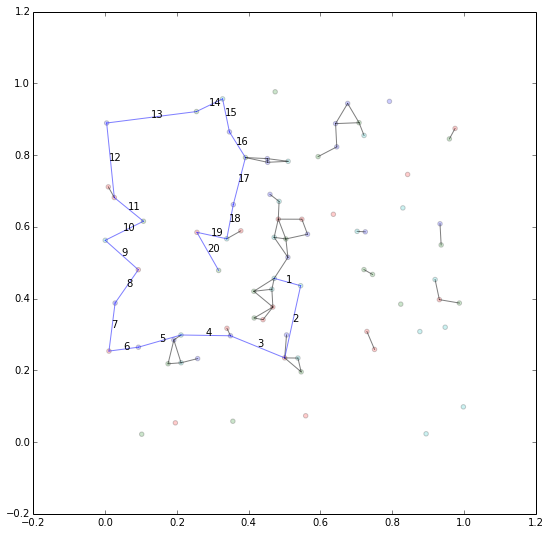
\includegraphics{output_79_0.png}

上のグラフで薄いグレーで描かれた線はノード間の距離が\(r\)より小さいために張られたエッジであり、これが連結しているひとまとまりがクラスターである。青色の線は、選ばれた意見同士をつなぐ(有向)エッジであり、振られている番号は時刻\(k\)に張られたエッジであることを表す。

このシミュレーションでは、考えるべき要素が二つある。1つは、\(r\)によって作られるクラスターに関する性質である。もうひとつは、選ばれた意見によって作られた軌跡に関するものである。ただし、それぞれが独立ではないために、完全に分けて考えることはできない。

まずは、閾値\(r\)と、意見の密度に関してクラスターがどのように形成されるかについての議論をしていくことにする。

閾値\(r\)を変えたときに意見の総数に対するクラスターの数との関係。横軸\(r\)、縦軸\(\phi = 1- (\text{クラスターの数})/(\text{意見の総数})\)の通常のプロット(上段)と両対数プロット(下段)。100回の試行の平均をとっている。

両対数プロットを見て分かるように、\(r\)の小さい領域では、ベキで近似することが出来そうであることが分かる。以下には、この両対数グラフの\(0<r<0.07\)の範囲を直線でフィッティングしたものを示す。このときの傾きは、およそ1.86であった。

また、これはS字型の曲線(シグモイド曲線)なので、その代表的な関数系である
\begin{gather}
\begin{split}\phi (r) = 1 - \exp \left[ -  \left( \frac{r}{\omega} \right)^{2} \right]\end{split}\notag
\end{gather}
としてパラメータ\(\omega\)に関して最小2乗法でフィッティングを行う。このとき、先ほどの場合とは異なり、\(r\)の比較的大きい領域のデータを含んでもよい。

先ほどのベキでフィッテイングした場合に比べて、大きい領域でもよくフィッティングできていること、それから関数系が
\begin{gather}
\begin{split}\phi (r) = 1 - \exp \left[ -  \left( \frac{r}{\omega} \right)^{2} \right]\end{split}\notag
\end{gather}
となっており、\(\phi = 1- (\text{クラスターの数})/(\text{意見の総数})\)の形との整合もとれていることから、この関数系に従うと考えても良いかもしれない。

次に、参加者の人数が変化したときに\(\phi\)がどう変化するかについて見てみることにする。このとき、総意見数と参加者の数、一人あたりの意見の数の間には比例の関係が成り立っており、参加者の数を増やすことと一人あたりの意見の数を増やすことはこの場合等価であるから、より細かく値を刻むことの出来る一人あたりの意見の数を変化させたときのクラスター数との間の関係について考えていく。

これらの量が解析的に求めることができないか、ということで計算をしてみた結果を以下に示すことにする。

点の分布する範囲は\(\Omega = [0,1]\times [0,1]\)であり、この中の面積\(S\)の領域の中に点を見出す確率は\(S\)である。

次に、領域内のある点\(\vec x=(x,y)\)を中心として半径\(r\)(\(0 < r \le 0.5\))の領域\(B(\vec x, r)\)内に点を見出す確率\(p(\vec x)\)は、境界の影響をうけない領域(\(\Omega ' = \{(x,y) | r \le x \le 1-r, r \le y \le 1-r \}\))では\(\pi r^{2}\)であり、境界の影響を受ける領域(\(\Omega'' = \Omega / \Omega'\))において点を見出す確率は、領域を
\begin{gather}
\begin{split}\begin{align}
\Omega''_{x} &= \{(x,y) | 0 \le x < r, r< y < 1-r\} \\
\Omega''_{1-x} &= \{(x,y) | 1-r < x \le 1, r< y < 1-r\} \\
\Omega''_{y} &= \{(x,y) | r < x < 1-r, 0 \le y < r\} \\
\Omega''_{1-y} &= \{(x,y) | r < x < 1-r, 1-r < y \le 1\} \\
\Omega''_{x,y} &= \{(x,y) | 0 \le x < r, 0 \le y < r\} \\
\Omega''_{1-x,y} &= \{(x,y) | 1-r < x \le 1, 0 \le y < r\} \\
\Omega''_{x,1-y} &= \{(x,y) | 0 \le x < r, 1-r < y \le 1\} \\
\Omega''_{1-x, 1-y} &= \{(x,y) | 1-r < x \le 1, 1-r < y \le 1\}
\end{align}\end{split}\notag
\end{gather}
のようにあらわすことにする(下図)。

図: 領域\(\Omega\)を分割した各領域

\(\Omega''_{i} = \{\Omega''_{x}, \Omega''_{1-x}, \Omega''_{y}, \Omega''_{1-y}\)\}、また\(\Omega''_{i,j} = \{\Omega''_{x,y}, \Omega''_{1-x,y}, \Omega''_{x,1-y}, \Omega''_{1-x,1-y}\}\)でまとめて書くことにすると、
\begin{gather}
\begin{split}p(r)_{\Omega''_{i}} = i \sqrt{r^{2}-i^{2}} + r^{2} \left[ \pi -\arccos \frac{i}{r} \right]\end{split}\notag
\end{gather}
図:
\(\vec{x} \in \Omega''_{x}\)であるときの面積\(S\)の求め方
\begin{gather}
\begin{split}\begin{align}p(r)_{\Omega''_{i,j}} = &\frac{1}{2}\left\{ \sqrt{r^{2}-i^{2}} + \min \left(j, \sqrt{r^{2}-i^{2}}\right) \right\}i + \frac{1}{2}\left\{ \sqrt{r^{2}-j^{2}} + \min \left( i, \sqrt{r^{2}-j^{2}}\right) \right\}j \\
&+ \frac{1}{2}r^{2} \left\{ 2\pi -\arccos \frac{i}{r}-\arccos \frac{j}{r}-\min \left( \frac{\pi}{2}, \arccos \frac{i}{r} +\arccos \frac{j}{r} \right) \right\}
\end{align}\end{split}\notag
\end{gather}
のようにあらわすことができる。

図:
\(\vec{x} \in \Omega''_{x,y}\)のときの面積\(S\)の求め方の一例。

確率\(p\)をすべての領域について積分した値は、領域\(\Omega\)から一様乱数によって一つの点を選び、その点を中心とした\(r\)による範囲に1つの点を見出す確率の期待値となる。

この確率を\(p'(r)\)とし、\(0\le r \le 0.5\)のときは
\begin{gather}
\begin{split}p'(r) = p'(r)_{\Omega''} + 4p'(r)_{\Omega''_{i}} + 4p'(r)_{\Omega''_{i,j}}\end{split}\notag
\end{gather}
とできる。それぞれの領域について積分を実行する。
\begin{gather}
\begin{split}p'(r)_{\Omega'} = \int_{r}^{1-r} \int_{r}^{1-r}\pi r^{2}\mathrm{d}x\mathrm{d}y = (1-2r)^{2}\pi r^{2}\end{split}\notag
\end{gather}\begin{gather}
\begin{split}\begin{align}
p'(r)_{\Omega'_{i}} = p'(r)_{\Omega'_{x}} &= \int_{0}^{r} \int_{r}^{1-r}\mathrm{d}x\mathrm{d}y\ x\sqrt{r^{2}-x^{2}} + r^{2}\left[\pi - \arccos\frac{x}{r}\right]\\
&= (1-2r)\left\{ \frac{r^{3}}{3} + r^{2}\pi\cdot r - r^{2}\cdot r \right\}\\
&= (1-2r)r^{3}\left( \pi-\frac{2}{3} \right)
\end{align}\end{split}\notag
\end{gather}
NOTE1:
\begin{gather}
\begin{split}\begin{align}
&\int_{0}^{r}\mathrm{d}x\ x\sqrt{r^{2}-x^{2}} \\
&\ \ \ \ \ \left[x = r\cos \theta \right]\\
&= \int_{\frac{\pi}{2}}^{0}\mathrm{d}\theta\ (-r\sin\theta)\ r\cos\theta\ r\sin\theta\\
&= r^{3}\left[ \frac{\sin^{3}\theta}{3}\right]^{\frac{\pi}{2}}_{0} \\
&= \frac{r^{3}}{3}
\end{align}\end{split}\notag
\end{gather}
NOTE2:

\(x = \cos t \ (0< t< \pi)\)とすると
\begin{gather}
\begin{split}\frac{\mathrm{d}x}{\mathrm{d}t} = - \sin t < 0\end{split}\notag
\end{gather}
\(t = \arccos x\)であるから、
\begin{gather}
\begin{split}\begin{align}
\frac{\mathrm{d}}{\mathrm{d}x}\arccos x &= \frac{1}{\frac{\mathrm{d}}{\mathrm{d}t}\cos t} = -\frac{1}{\sin t}\\
&=- \frac{1}{\sqrt{\sin^{2}t}} = - \frac{1}{\sqrt{1- \cos^{2}t}} \\
&= - \frac{1}{\sqrt{1- x^{2}}}
\end{align}\end{split}\notag
\end{gather}
したがって、
\begin{gather}
\begin{split}\begin{align}
\int \arccos x \mathrm{d}x\  &= x\arccos x + \int \frac{x}{\sqrt{1-x^{2}}}\mathrm{d}x\\
&=x\arccos x - \sqrt{1-x^{2}} + C
\end{align}\end{split}\notag
\end{gather}
(\(C\)は積分定数)

今の場合、
\begin{gather}
\begin{split}\begin{align}
\int^{r}_{0} \arccos \frac{x}{r} \mathrm{d}x &= \int^{1}_{0}\arccos t \cdot r\mathrm{d}t\\
&= r \left[ t \arccos t - \sqrt{1-t^{2}} \right]^{1}_{0}\\
&= r ( 1\arccos1 -\sqrt{1-1} - 0 \arccos0 + \sqrt{1-0})\\
&= r
\end{align}\end{split}\notag
\end{gather}
\(p'(r)_{\Omega''_{i,j}}\)を以下のように分解してそれぞれ計算する。
\begin{gather}
\begin{split}\begin{align}
p'(r)_{\Omega''_{i,j}} &= p'(r)_{\Omega''_{x, y}}\\
&= p'(r)_{\Omega''_{x, y}1}  +p'(r)_{\Omega''_{x, y}2}\\
&= p'(r)_{\Omega''_{x, y}1'} - p'(r)_{\Omega''_{x, y}1''} + p'(r)_{\Omega''_{x, y}2}
\end{align}\end{split}\notag
\end{gather}\begin{gather}
\begin{split}\begin{align}
p'(r)_{\Omega''_{x,y}1'} &= \int^{r}_{0}\int^{r}_{0}\mathrm{d}x\mathrm{d}y\ x\sqrt{r^{2}-x^{2}} + y \sqrt{r^{2} -y^{2}} + \frac{1}{2}r^{2}\left( 2\pi -2\arccos\frac{x}{r} -2\arccos\frac{y}{r} \right) \\
&= r\int^{r}_{0}\mathrm{d}x\ \left\{x\sqrt{r^{2}-x^{2}} - r^{2}\arccos\frac{x}{r} \right\}
+ r\int^{r}_{0}\mathrm{d}x\ \left\{x\sqrt{r^{2}-x^{2}} - r^{2}\arccos\frac{x}{r} \right\} + \pi r^{2}\cdot r^{2}\\
&= r\left( \frac{r^{3}}{3} -r^{3} \right) + r\left( \frac{r^{3}}{3} -r^{3} \right) + \pi r^{4}\\
&=  \left(\pi -\frac{4}{3}\right)r^{4}
\end{align}\end{split}\notag
\end{gather}\begin{gather}
\begin{split}\begin{align}
p'(r)_{\Omega''_{x,y}1''} &= \int^{r}_{0}\int^{\sqrt{r^{2}-x^{2}}}_{0}\mathrm{d}x\mathrm{d}y\ \left[ x\sqrt{r^{2}-x^{2}} + y \sqrt{r^{2} -y^{2}} + r^{2}\left(\pi -\arccos\frac{x}{r} -\arccos\frac{y}{r}\right) \right]\\
&= \int^{r}_{0}\mathrm{d}x\left[ \left\{ x\sqrt{r^{2}-x^{2}} + r^{2}\pi -r^{2}\arccos\frac{x}{r} \right\}\sqrt{r^{2}-x^{2}} + \int^{\sqrt{r^{2}-x^{2}}}_{0}\mathrm{d}y\ y\sqrt{r^{2}-y^{2}} -r^{2}\arccos\frac{y}{r}\right]\\
&= \int^{r}_{0}\mathrm{d}x\left[ x(r^{2}-x^{2}) + r^{2}\pi\sqrt{r^{2}-x^{2}} -r^{2}\arccos \frac{x}{r} \sqrt{r^{2}-x^{2}} + \frac{r^{3}}{3} - \frac{x^{3}}{3} - r^{2}\frac{\pi}{2}\sqrt{r^{2}-x^{2}} + r^{2}\arccos\frac{x}{r}\sqrt{r^{2}-x^{2}} +r^{2}x - r^{3}\right] \\
&= \int^{r}_{0}\mathrm{d}x \left[-\frac{4}{3}x^{3} + 2r^{2}x - \frac{2}{3}r^{3} + \frac{\pi}{2}r^{2}\sqrt{r^{2}-x^{2}} \right]\\
&= \left[ -\frac{4}{3}\frac{x^{4}}{4} + r^{2}x^{2} - \frac{2}{3}r^{3}x \right]^{r}_{0} + \frac{\pi}{2}r^{2}\cdot \frac{1}{4}\pi r^{2}\\
&= -\frac{r^{4}}{3} + r^{4} -\frac{2}{3}r^{4} + \frac{\pi ^{2}}{8}r^{4}\\
&= \frac{\pi^{2}}{8}r^{4}
\end{align}\end{split}\notag
\end{gather}
NOTE1:

\(y=r\cos \theta\)とおく。

\(y\)の積分領域\([0, \sqrt{r^{2}-x^{2}}]\)は\(\theta\)の範囲としては\([\pi/2, \theta' = \arcsin(x/r)]\)となる。

(図)
\begin{gather}
\begin{split}\begin{align}
\int^{\sqrt{r^{2}-x^{2}}}_{0}\mathrm{d}y\ y\sqrt{r^{2}-y^{2}} &= \int^{\theta'}_{\frac{\pi}{2}}-r^{3}\sin^{2}\theta\ \cos\theta \mathrm{d}\theta\\
&= r^{3}\left[ \frac{\sin^{3}\theta}{3} \right]^{\frac{\pi}{2}}_{\theta'}\\
&= \frac{r^{3}}{3} - r^{3}\frac{\left( \frac{x}{r} \right)^{3}}{3}\\
&= \frac{r^{3}}{3} - \frac{x^{3}}{3}
\end{align}\end{split}\notag
\end{gather}
NOTE2:

\(t = x/r\)とおいて積分する。
\begin{gather}
\begin{split}\begin{align}
r^{2}\int^{\sqrt{r^{2}-x^{2}}}_{0}\mathrm{d}y\ \arccos \frac{y}{r} &= r^{2}\int^{\frac{\sqrt{r^{2}-x^{2}}}{r}}_{0}r\mathrm{d}t\ \arccos t\\
&= r^{3}\left[ t\arccos t - \sqrt{1-t^{2}} \right]^{\frac{\sqrt{r^{2}-x^{2}}}{r}}_{0}\\
&= r^{3}\left[ \frac{\sqrt{r^{2}-x^{2}}}{r}\left( \frac{\pi}{2} - \arcsin \frac{x}{r} \right) - \frac{x}{r} + 1 \right]\\
&= r^{2}\frac{\pi}{2}\sqrt{r^{2}-x^{2}} - r^{2}\sqrt{r^{2}-x^{2}}\arccos\frac{x}{r} - r^{2}x + r^{3}
\end{align}\end{split}\notag
\end{gather}\begin{gather}
\begin{split}\begin{align}
p'(r)_{\Omega''_{x, y}2} &= \int^{r}_{0}\int^{r}_{0}\mathrm{d}x\mathrm{d}y\ \frac{1}{2}x\sqrt{r^{2}-x^{2}} + \frac{1}{2}y\sqrt{r^{2} -y^{2}} + xy + \frac{1}{2}r^{2}\left( 2\pi - \arccos\frac{x}{r} - \arccos\frac{y}{r} - \frac{\pi}{2} \right)\\
&= \int^{r}_{0}\mathrm{d}x\int^{\sqrt{r^{2}-x^{2}}}_{0}\mathrm{d}y\ \frac{1}{2}x\sqrt{r^{2}-x^{2}} + \frac{1}{2}y\sqrt{r^{2} -y^{2}} + xy + \frac{1}{2}r^{2}\left( 2\pi - \arccos\frac{x}{r} - \arccos\frac{y}{r} - \frac{\pi}{2} \right)\\
&= \int^{r}_{0}\mathrm{d}x\left[ \left\{ \frac{1}{2}x\sqrt{r^{2}-x^{2}} + \frac{3}{4}\pi r^{2} - \frac{1}{2}r^{2}\arccos\frac{x}{r} \right\}\sqrt{r^{2}-x^{2}} + \int^{\sqrt{r^{2}-x^{2}}}_{0}\mathrm{d}y\ \frac{1}{2}y\sqrt{r^{2}-y^{2}} + xy - \frac{1}{2}r^{2}\arccos\frac{y}{r}\right]\\
&= \int^{r}_{0}\mathrm{d}x\left[ \frac{1}{2}xr^{2} - \frac{x^{3}}{2} + \frac{3}{4}\pi r^{2}\sqrt{r^{2}-x^{2}} - \frac{1}{2}r^{2}\arccos \frac{x}{r} \sqrt{r^{2}-x^{2}} \right.\\
&\ \ \ \ \ \ \ \ \ \ + \left. \frac{r^{3}}{6} - \frac{x^{3}}{6} + \frac{1}{2}xr^{2} - \frac{x^{3}}{2} - \frac{\pi}{4}r^{2}\sqrt{r^{2}-x^{2}} + \frac{1}{2}r^{2}\arccos\frac{x}{r}\sqrt{r^{2}-x^{2}} + \frac{1}{2}r^{2}x - \frac{r^{3}}{2}\right] \\
&= \int^{r}_{0}\mathrm{d}x\left[- \frac{7}{6}x^{3} - \frac{r^{3}}{3} + \frac{3}{2}r^{2}x + \frac{\pi}{2}r^{2}\sqrt{r^{2}-x^{2}} \right]\\
&= -\frac{7}{24}r^{4} - \frac{r^{4}}{3} + \frac{3}{4}r^{4} + \frac{\pi}{2}r^{2}\cdot \frac{\pi}{4}r^{2}\\
&= \left( - \frac{7}{24} - \frac{1}{3} + \frac{3}{4} + \frac{\pi^{2}}{8}\right)r^{4}\\
&= \left( \frac{\pi^{2}}{8} + \frac{1}{8} \right)r^{4}
\end{align}\end{split}\notag
\end{gather}\begin{gather}
\begin{split}\begin{align}
p'(r)_{\Omega''_{i,j}} &= p'(r)_{\Omega''_{x, y}}\\
&= p'(r)_{\Omega''_{x, y}1}  +p'(r)_{\Omega''_{x, y}2}\\
&= p'(r)_{\Omega''_{x, y}1'} - p'(r)_{\Omega''_{x, y}1''} + p'(r)_{\Omega''_{x, y}2}\\
&= \left(\pi -\frac{4}{3}\right)r^{4} - \frac{\pi^{2}}{8}r^{4} + \left( \frac{\pi^{2}}{8} + \frac{1}{8} \right)r^{4}\\
&= \left(\pi -\frac{29}{24}\right)r^{4}
\end{align}\end{split}\notag
\end{gather}
これまでの結果をすべて合わせると、
\begin{gather}
\begin{split}\begin{align}
p'(r) &= p'(r)_{\Omega''} + 4p'(r)_{\Omega''_{i}} + 4p'(r)_{\Omega''_{i,j}}\\
&= (1-2r)^{2}\pi r^{2} + (1-2r)r^{3}\left( 4\pi-\frac{8}{3} \right) + \left(4\pi -\frac{29}{6}\right)r^{4}\\
&= \pi r^{2} - 4\pi r^{3} + 4\pi r^{4} + 4\pi r^{3} -\frac{8}{3}r^{3} - 8\pi r^{4} + \frac{16}{3}r^{4} + 4\pi r^{4} - \frac{29}{6}r^{4}\\
&= \frac{1}{2}r^{4} -\frac{8}{3}r^{3} + \pi r^{2}
\end{align}\end{split}\notag
\end{gather}
を得る。

以下に\(r\)を\(0.01\)から\(0.5\)まで変えたとき、領域\(\Omega\)上に選ばれた1つの点からいくつのエッジが結ばれるか(次数)の期待値を求め、この試行を100回繰り返して平均をとった。このときの値はグラフでは青色の曲線であらわされている。一方、先程までの議論の結果として、\(\Omega\)上にとった1つの点のまわりの\(r\)による範囲に他の点が存在する確率の期待値は
\begin{gather}
\begin{split}p'(r) = \frac{1}{2}r^{4} -\frac{8}{3}r^{3} + \pi r^{2}\end{split}\notag
\end{gather}
で表すことができた。よって、一番はじめの例で数直線上で考えたときと同じように、次数の期待値は二項分布\(B(k,p'(r))\)で表すことができるから、意見空間全体にある点の個数を\(M\)とすると、ある\(r'\)における平均次数は\(p'(r')(M-1)\)で表せる。グラフ上では緑色の曲線でこのグラフが示されている。このときの分散\(\sigma^{2}\)は、\(p'(r')(1-p'(r'))M\)である。この分散は1回の試行に関するものであったので、さらに100回の試行を行った今回の偏差\(\sigma'\)は\(\sigma/\sqrt{100}\)である。この範囲を示したものが、グラフの中の緑色の透過処理を施した範囲である。

グラフからも、解析的に計算した上の結果が実際に測った量とよく一致していることが分かる。

図: \(r\)とクラスターの平均次数の関係


\section{意見間距離の平均値と人数\(N\)との間の関係}
\label{draft:id9}
実際にはこれまで考えたクラスターから1つの意見が代表して選ばれ、時間が1進むごとに、そこから一番近い位置にあるクラスターからまた1つ意見が選ばれていくような過程を考えているので、選ばれた意見から構成されるネットワークは、単純に一本の線状に乗るようなネットワークを構成する。したがって、一般的なネットワークの特徴量ではなく、意見空間という位置の情報を含めたものであることを利用して、1つの意見ごとの平均距離(ネットワーク科学でいうところのノード間距離とは異なるものであることに注意)を測り、これが会議の参加人数とどのような関係であるかを見ていくことにする。

以下のグラフは、一人あたりの意見の数\(S=20\)、意見のクラスタ化閾値\(r=0.07\)としたときの、参加者の人数\(N\)と選ばれた意見間の距離の平均値\(l\)の関係を示したものである。

図: 意見間の距離の平均値と人数\(N\)の間の関係

このグラフを見て分かるように、\(l\)は\(N\)の関数として見たとき下に凸な関数となっており、この\(l\)と会議の質との間に負の相関があるとすれば、この\(l\)は人数と会議の質の間の関係を示す指標となりうることが分かる。

さて、このようなグラフとなるのは、先程まで考えたように人の数が増えると意見の密度が大きくなり、同じ\(r\)でも、クラスターの融合が進むので、結果的にクラスター間の距離は離れることとなるということと、意見の密度が小さいときには、クラスターは形成されにくいが、逆に意見間の距離は広がるために、選ばれた意見間の距離も大きくなることになる。

また、今回は横軸の変数として人の数\(N\)を変更させていったが、参加者の発言頻度が会議の質との関係がないと仮定した場合には、一人あたりの意見の数\(S\)を変えた場合と完全に等価になる。すなわち、横軸に\(M=S\times N\)としてグラフを描くこともできる。

はじめに考えたように、このように意見空間において意見のクラスター化を行うということは、近すぎる内容の意見は人は発言しないということを意味しており、この結果、参加する人数が大きいほど、それぞれの人がいいそうなことが予想されるので、当人としては当然の流れとして、一つ前の意見から離れた意見を選ぶことが許されることになる。しかし、あまりに意見間の距離が大きくなると、参加している人の考えるつながりとは必ずしも一致しないので、そこに意見の飛躍が生じることによって「わからない意見」が増えることになる。一方で人の数が少なく、それぞれの意見の間に差が生じている時には、そもそも意見の間の差が大きいために、意見同士はつながりが小さくなる。


\subsection{結論}
\label{draft:id10}
いくつかの簡単なモデルを考え、それぞれの場合についての計算とシミュレーションを行った。はじめに作成したモデルについては、人数との間の関連が得られていなかったために、このモデル自体ではシステムサイズと効率というものを議論するのには不十分であると見ることができる。しかしながら、ここで見たように、当然人の発現頻度というものに着目すれば、これを効率とみなして議論を進めることも可能であると思う。二つ目に考えたモデルでは、参加者間の差異をはじめから考慮せずに、問題となるのは意見間の関係であるとして問題を簡単化した。ぞれぞれの最も近い意見を持ち寄り、その順番にそれぞれの発言確率に従っていく場合を考えることにしている。この結果は人の数\(N\)が大きくなると、得られた意見のネットワークにおける各ステップの平均の距離が、\(N\)が大きくになるにつれて小さくなるというものである。この結果自体はごく当たり前のことを述べただけのものであるが、しかし実際には人の数と要素の数の間の関係は完全に等価ではないので(人の数が増えるということは、発言確率\(p\)が小さい時でも、誰かが発言するということであり、一人あたりの意見の数\(S\)が大きいこととは違った結果となる可能性がある)、



\renewcommand{\indexname}{Index}
\printindex
\end{document}
